\documentclass{article}

\usepackage{graphicx}
\usepackage{hyperref}
\usepackage{xcolor}
\usepackage[T1]{fontenc}

\title{Students Independent Study 1}
\author{Amangeldi Zhanserik}
\date{05 02 2005}

\begin{document}

\begin{titlepage}
    \centering

    \vspace*{1cm}

    \rule{\textwidth}{1pt}

    \vspace{2\baselineskip}

    {\huge  Cyber Security } \\

    \vspace{1\baselineskip}

    {\huge \textbf{ Lab 2 - Online Malware Investigation Tools }}

    \vspace{2\baselineskip}

    \rule{\textwidth}{1pt}

    \vspace{1cm}

    \large

    \begin{flushleft}
        \begin{minipage}{.8\textwidth}
            \raggedright
            Fullname: Amangeldi Zhanserik \\
            ID: 22B030301 \\
            E-mail: {\normalsize \url{zha_amangeldi@kbtu.kz}} \\
            Date of submission: 05/02/2025 \\
            Class time: Thursday, 15:00--18:00 \\
        \end{minipage}%
    \end{flushleft}

    \vspace{2cm}

    
\includegraphics[width=.7\textwidth]{logo-kbtu.png}

    \vfill

    School of Information System and Engineering \\
    Kazakh-British Technical University \\
    Academic Year 2024-2025 \\
\end{titlepage}

\section*{Part 1: Perform Static Malware Analysis}

In this part, I submitted a file hash to an online service that looked up the hash and returned information about the associated malware file. The file hash is a computed representation, or fingerprint, for a file. File hashes are unique and extremely difficult to duplicate.

\subsection*{Step 1: Submit the hash.}

\raggedright{I submitted this \textbf{05383088d0d46a5b5f4de852703601a6c39f04844ab63a1850197fcb011f3c81} hash to the \textbf{VirusTotal} website. The website returned information about the malware file associated with the hash.}

\vspace{2\baselineskip}

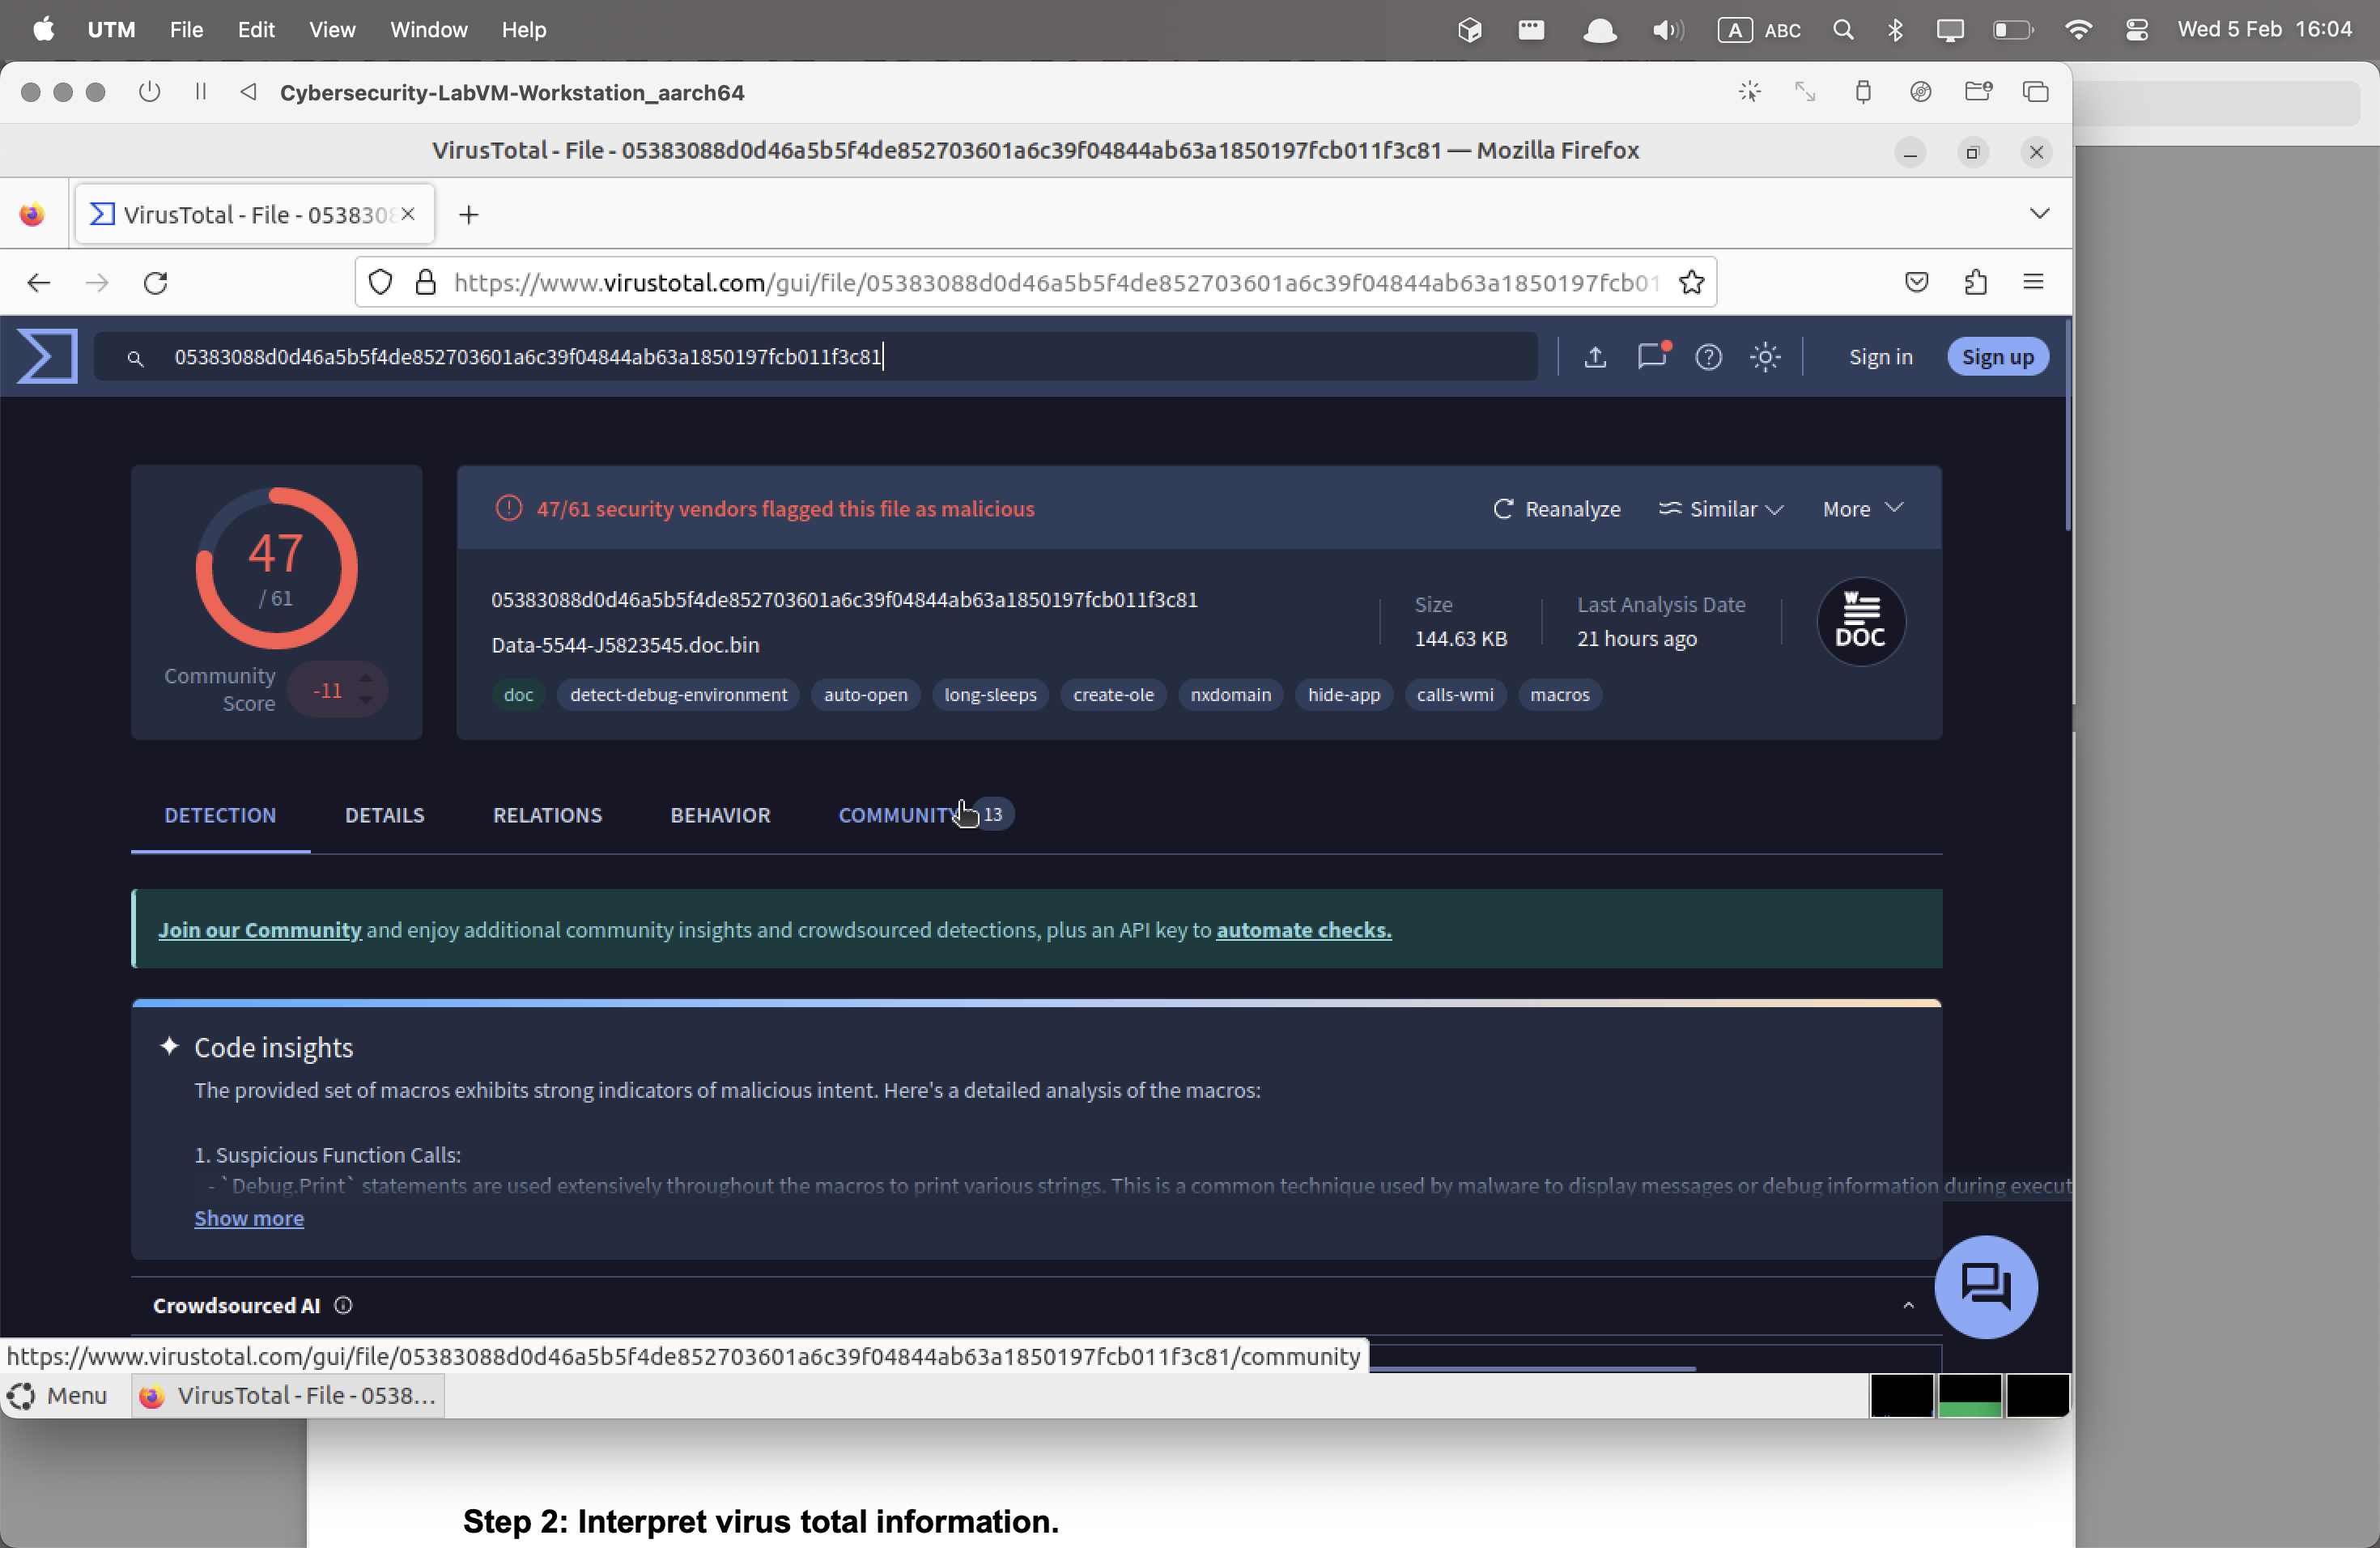
\includegraphics[width=1\textwidth]{1.png}

\subsubsection*{Question and Answer}
\textbf{\colorbox{yellow}{QUESTION 1: }}Has malware entered the XYZ, Inc. network? \\
\textbf{Answer: } No, malware has not entered the XYZ, Inc. network.

\vspace{1\baselineskip}

\textbf{\colorbox{yellow}{QUESTION 2: }}In your job, what should you do now? \\
\textbf{Answer: } I should investigate the source of the file and ensure that no other malicious files are present on the network. Additionally, I should update the antivirus software and perform a full system scan to ensure that the system is secure.

\newpage

\subsection*{Step 2: Interpret virus total information.}

\textbf{\colorbox{yellow}{Question 1: }} How many of the antivirus products flagged the file as malicious? What does this tell you about the
reliability of antivirus programs? \\
\textbf{Answer: } 47 antivirus products flagged the file as malicious. This indicates that the file is likely malicious and that antivirus programs are reliable.

\vspace{1\baselineskip}

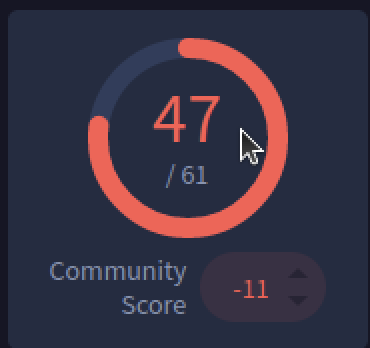
\includegraphics[width=0.5\textwidth]{2.png}

\vspace{2\baselineskip}

\textbf{\colorbox{yellow}{Question 2: }} What type of file has the malware been identified as? \\
\textbf{Answer: } Word DOC file. 

\vspace{1\baselineskip}

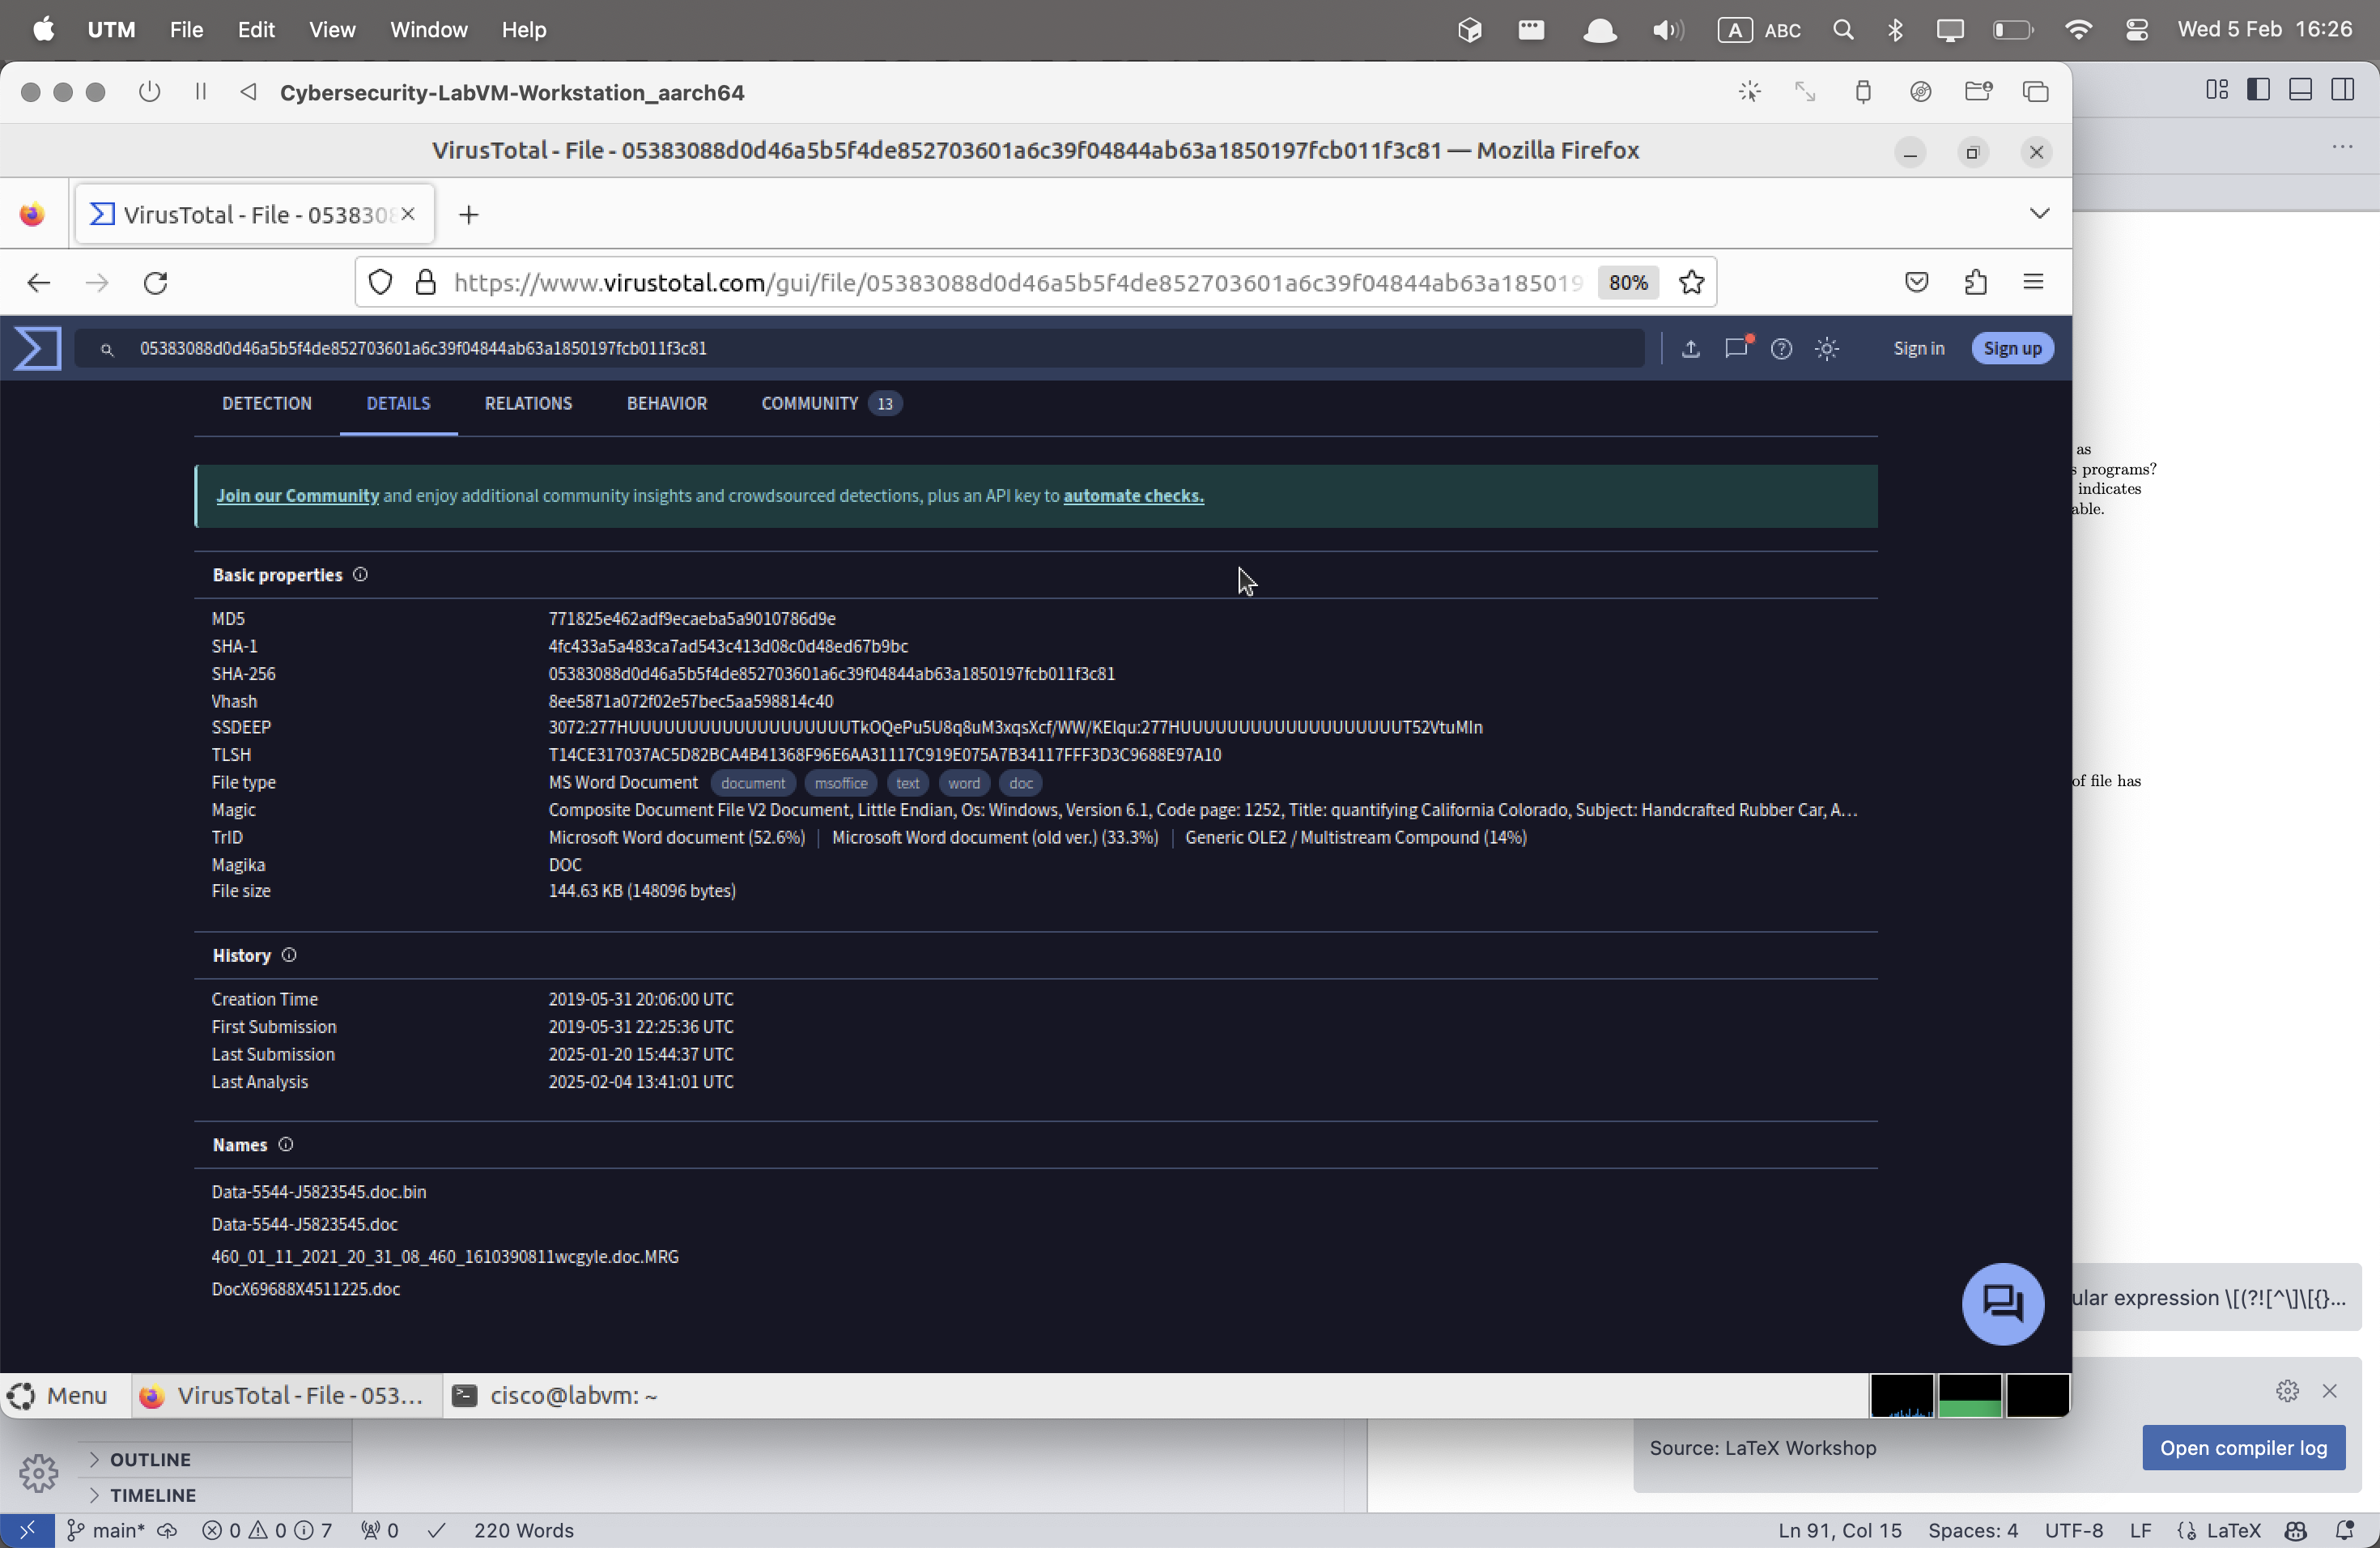
\includegraphics[width=1\textwidth]{3.png}

\vspace{2\baselineskip}

\textbf{\colorbox{yellow}{Question 3: }} What is the first Domain that the malware makes an HTTP request to? \\
\textbf{Answer: } \textcolor{blue}{http://ab.fitzio.com}

\vspace{1\baselineskip}

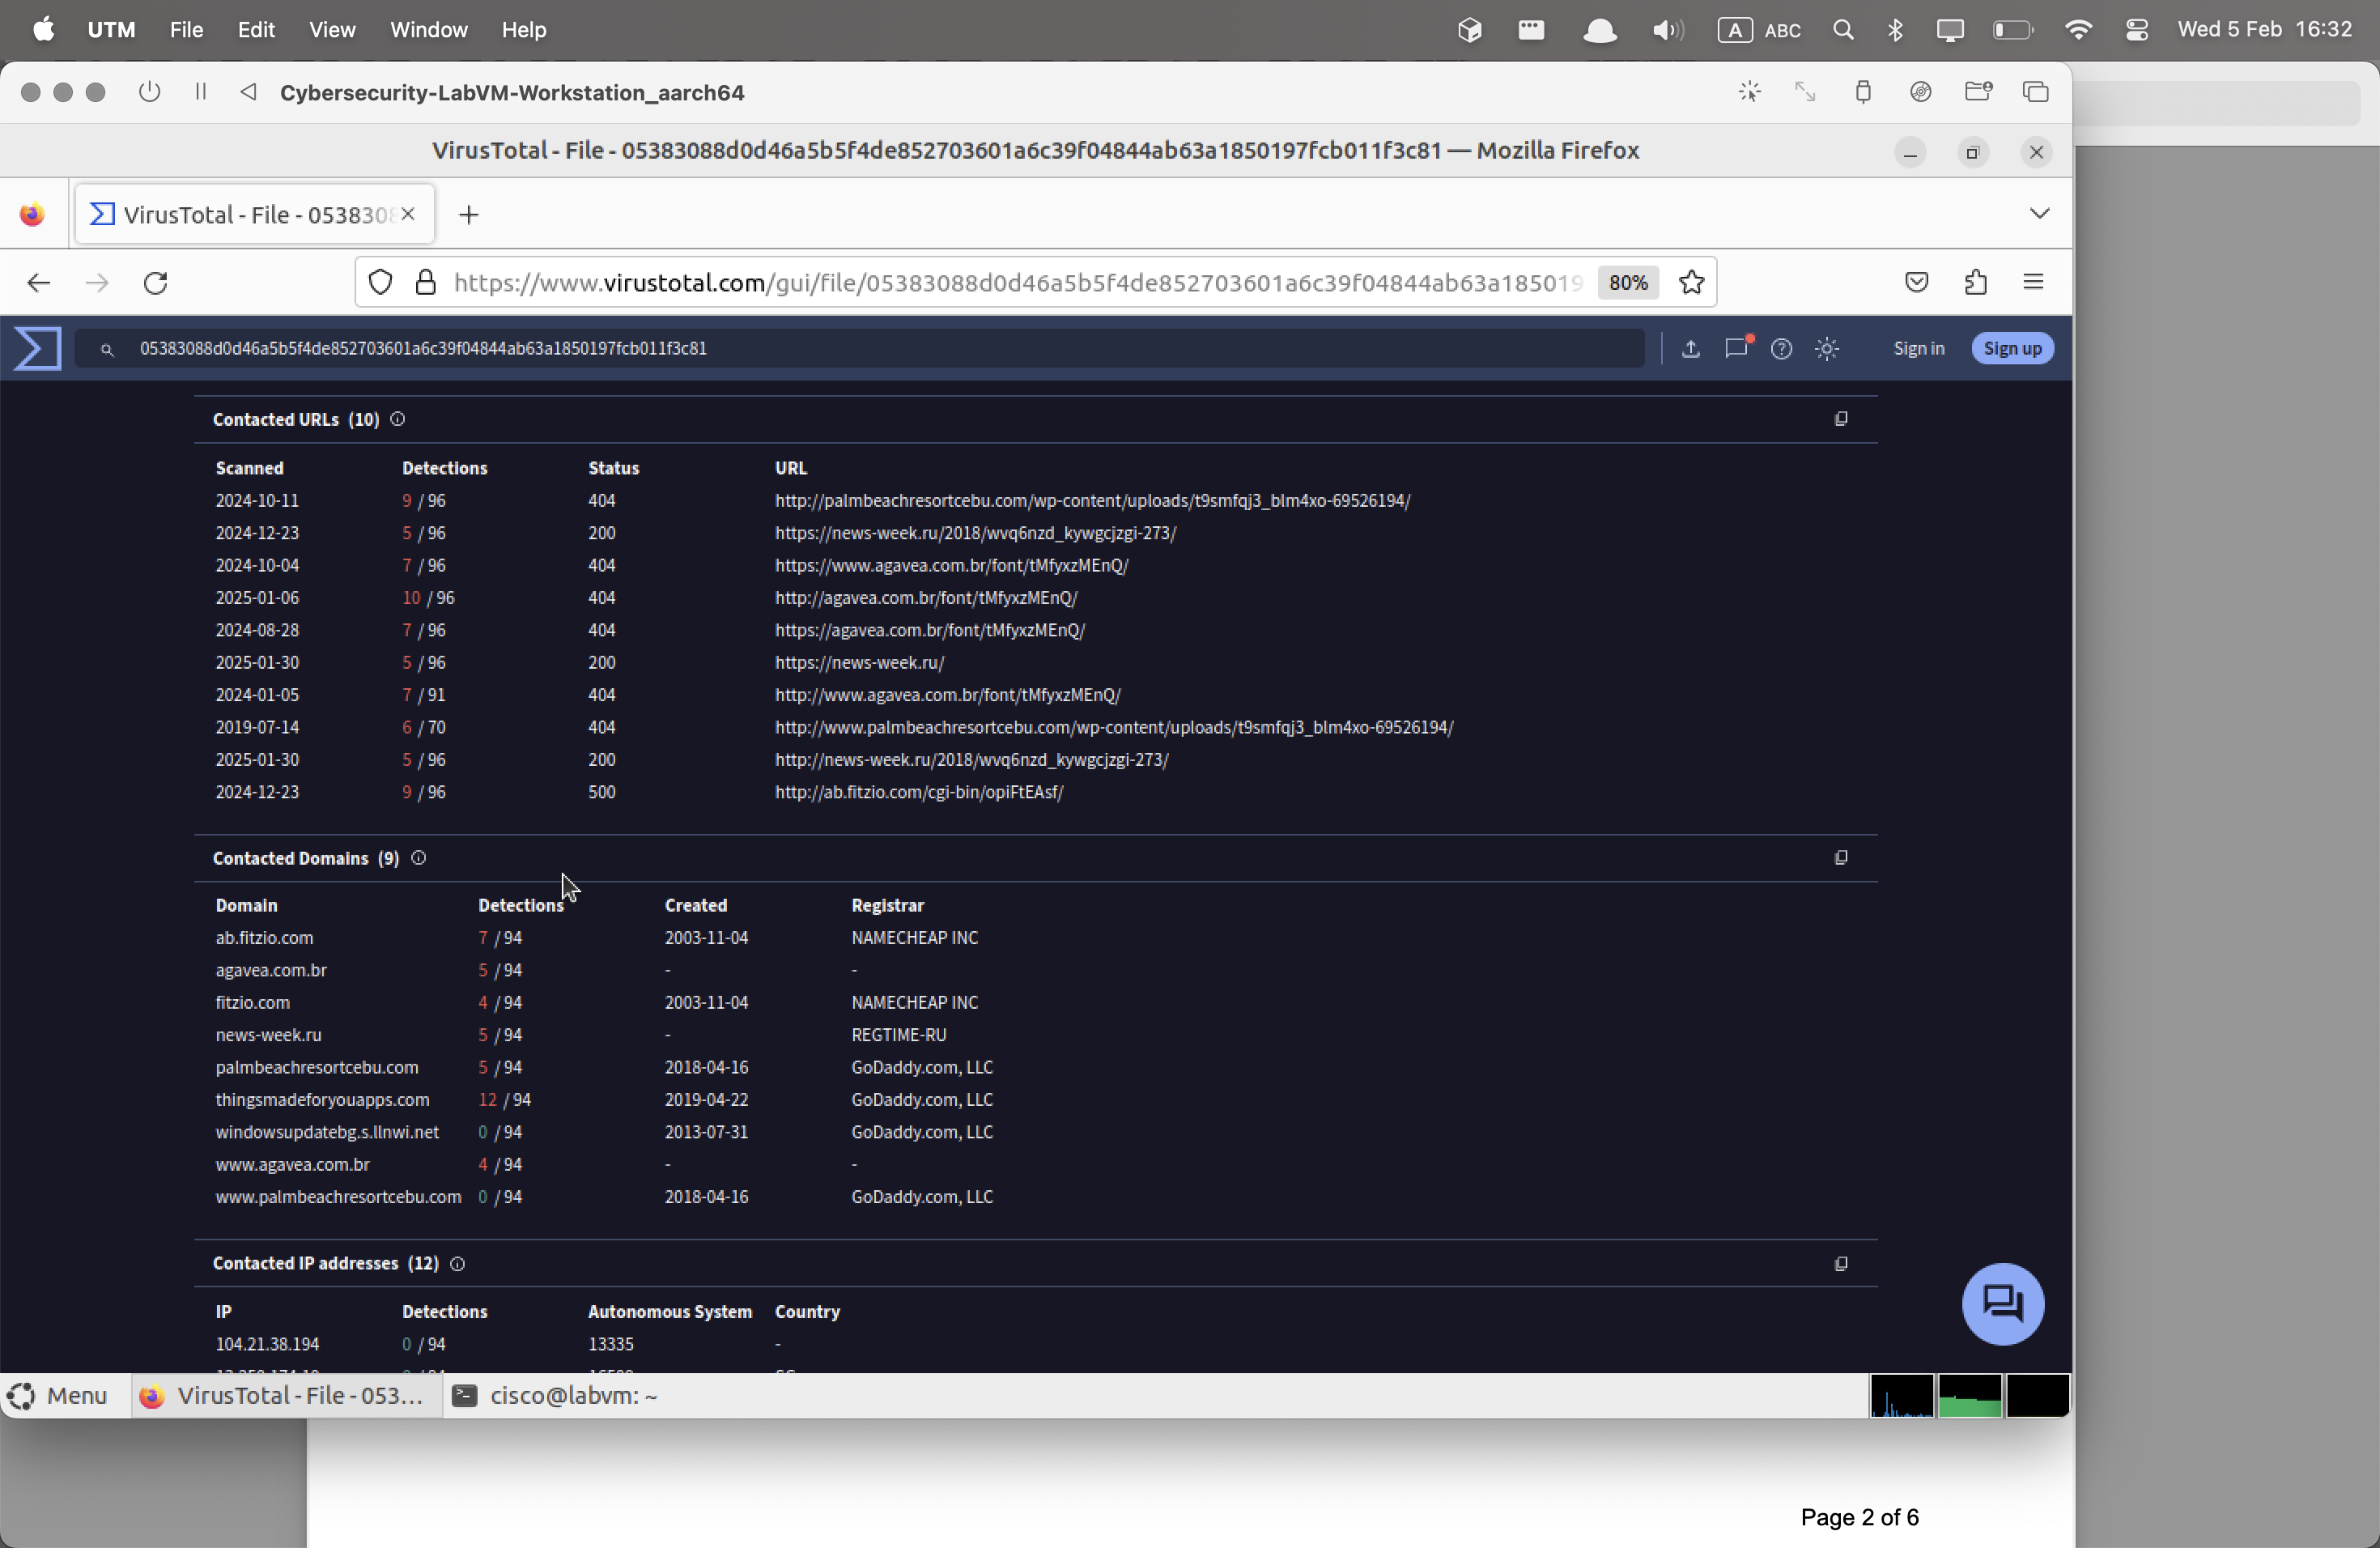
\includegraphics[width=1\textwidth]{4.png}

\vspace{1\baselineskip}

\textbf{\colorbox{yellow}{Question 4: }} What is unusual about that value? \\
powershell -nop -e JABSADMAWgB0AE...

\vspace{1\baselineskip}

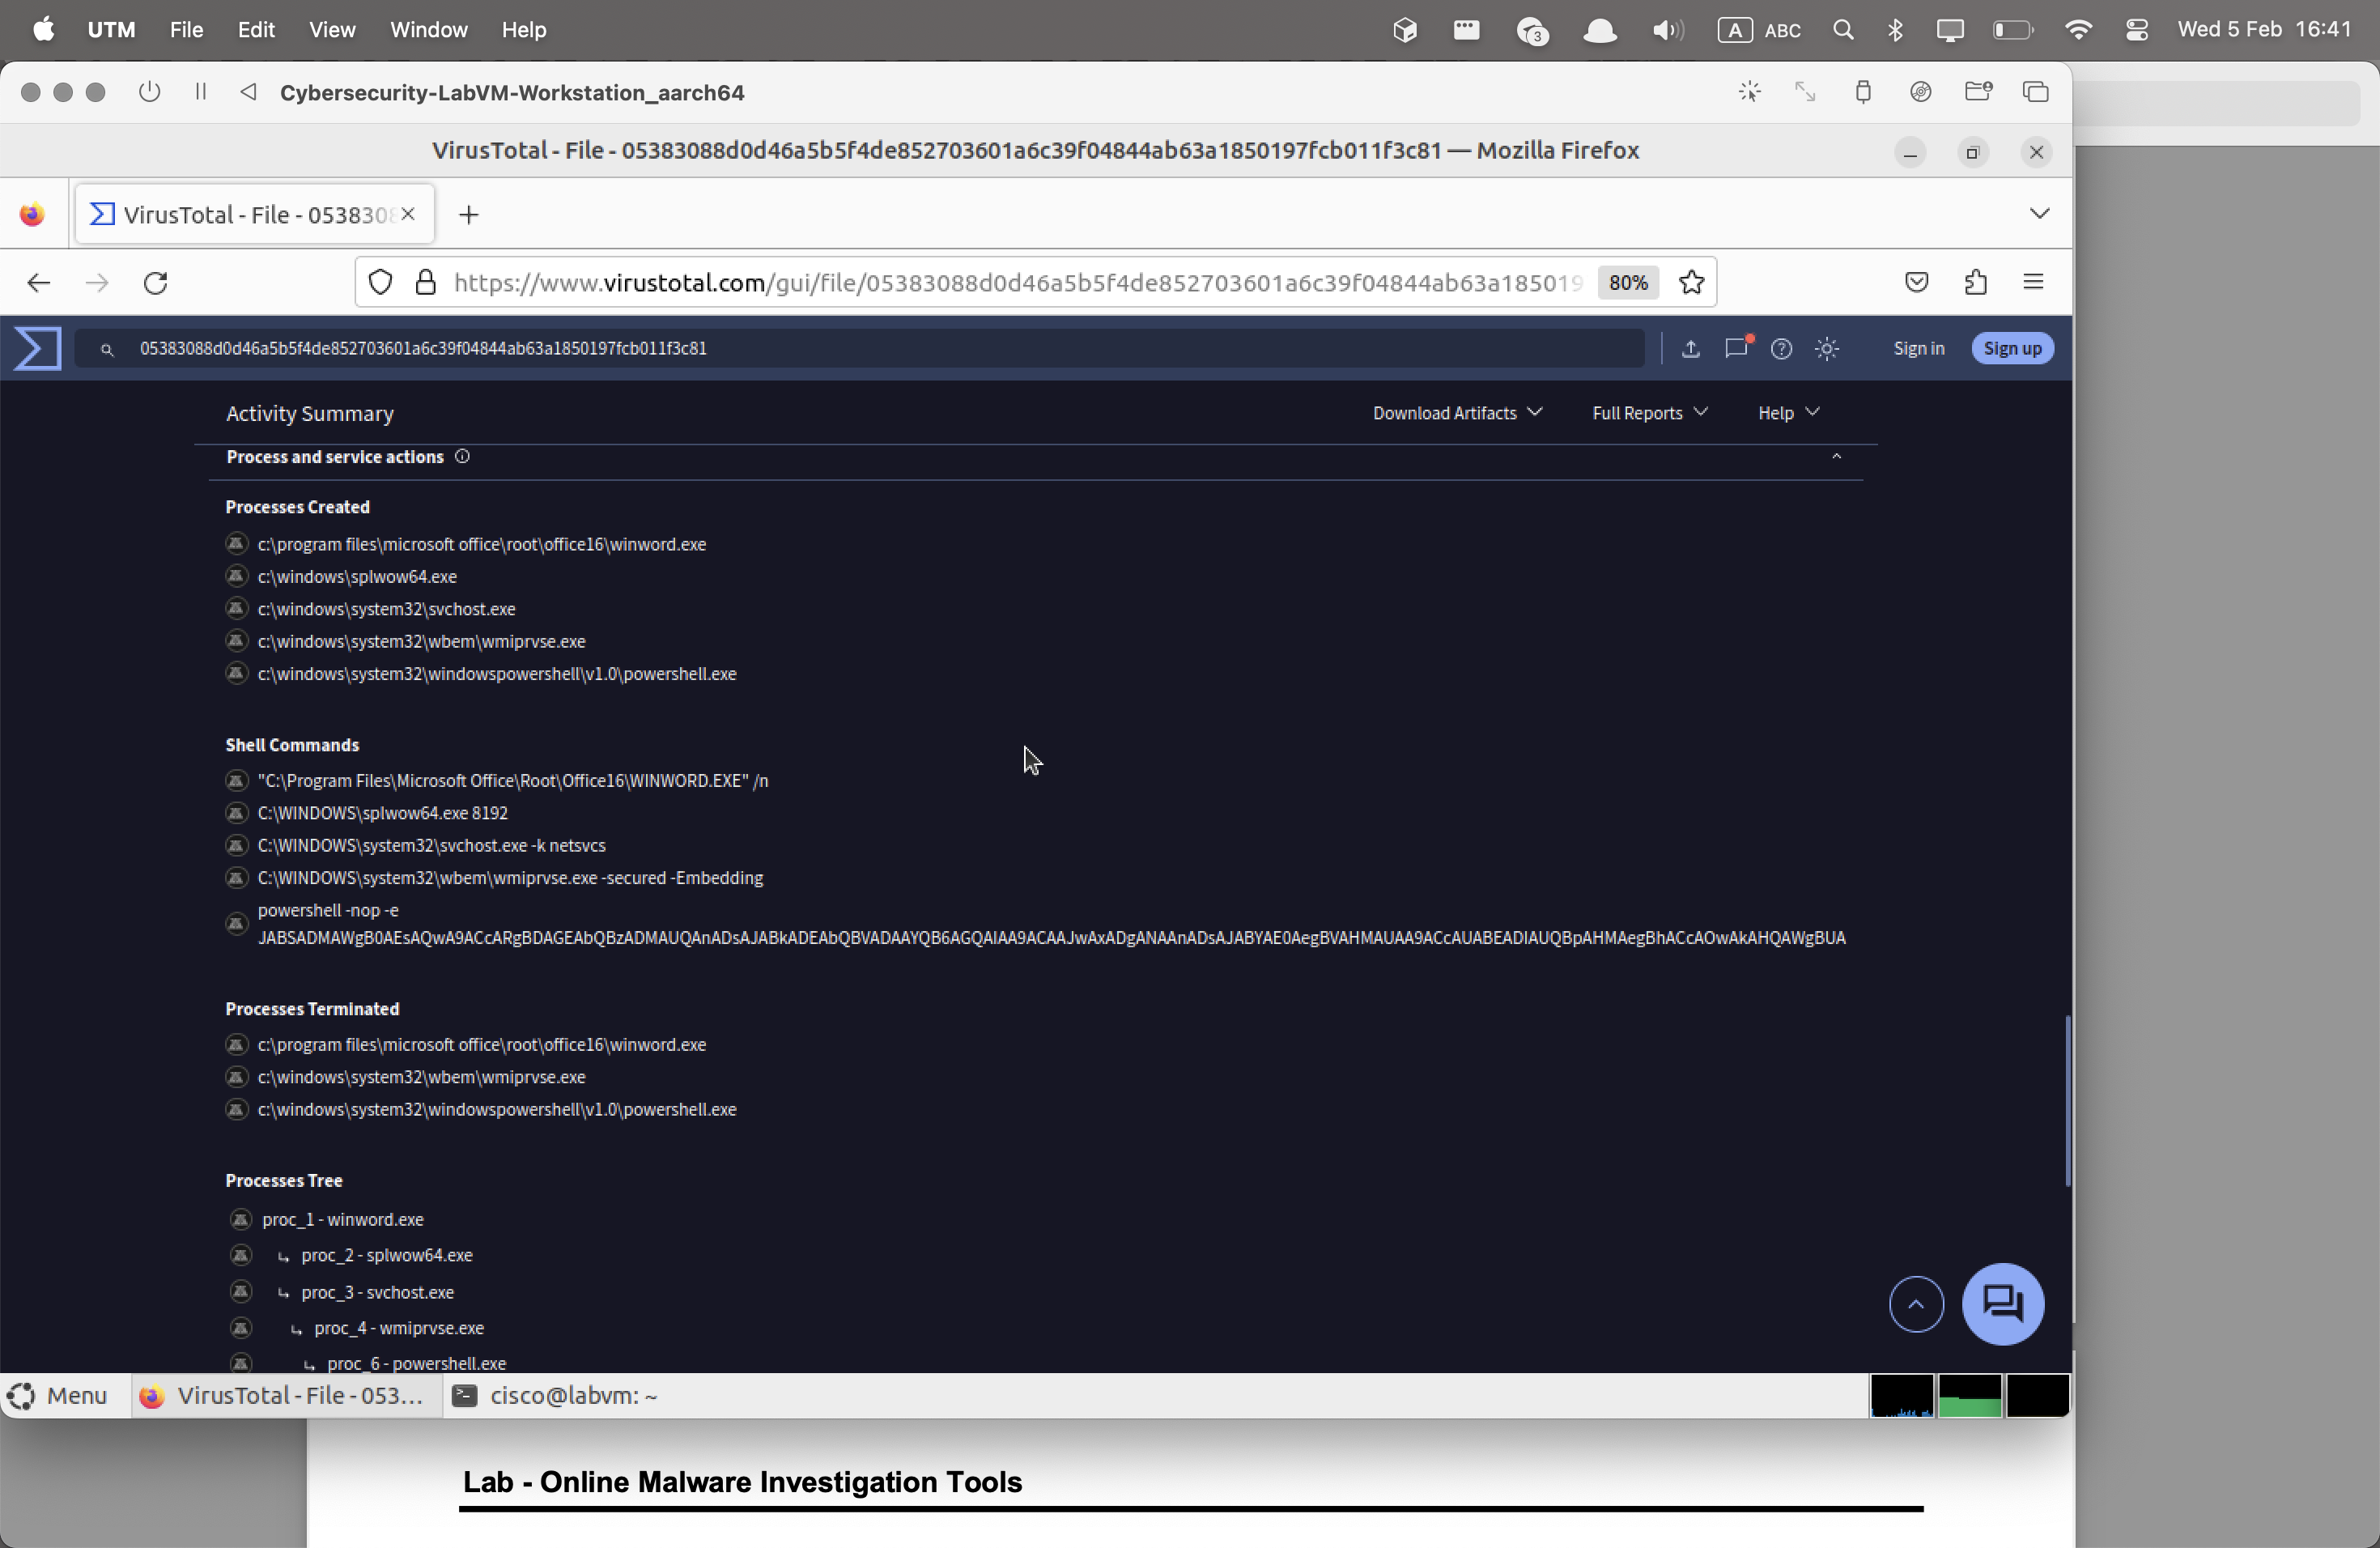
\includegraphics[width=1\textwidth]{5.png}

\newpage

\textbf{\colorbox{yellow}{Question 5: }} What are YARA signatures? \\
\textbf{Answer: } YARA signatures are a way to identify and classify malware by creating rules that describe patterns of malicious behavior or characteristics within files. These rules can be used to scan files and detect malware based on specific patterns, strings, or binary sequences.

\vspace{1\baselineskip}

\textbf{\colorbox{yellow}{Question 6: }} From the description fields in the YARA signatures, what can you learn about how the malware uses PowerShell? \\
\textbf{Answer: } The malware uses Powershell to encode the hash and after that run script got by encoding.

\vspace{2\baselineskip}


\includegraphics[width=1\textwidth]{6.png}

\newpage

\section*{Part 2: Perform Dynamic Malware Analysis}

\subsection*{Step 1: Access ANY.RUN and Submit IOC}

I checked this website and submit hash what we have and get this result.

\vspace{1\baselineskip}
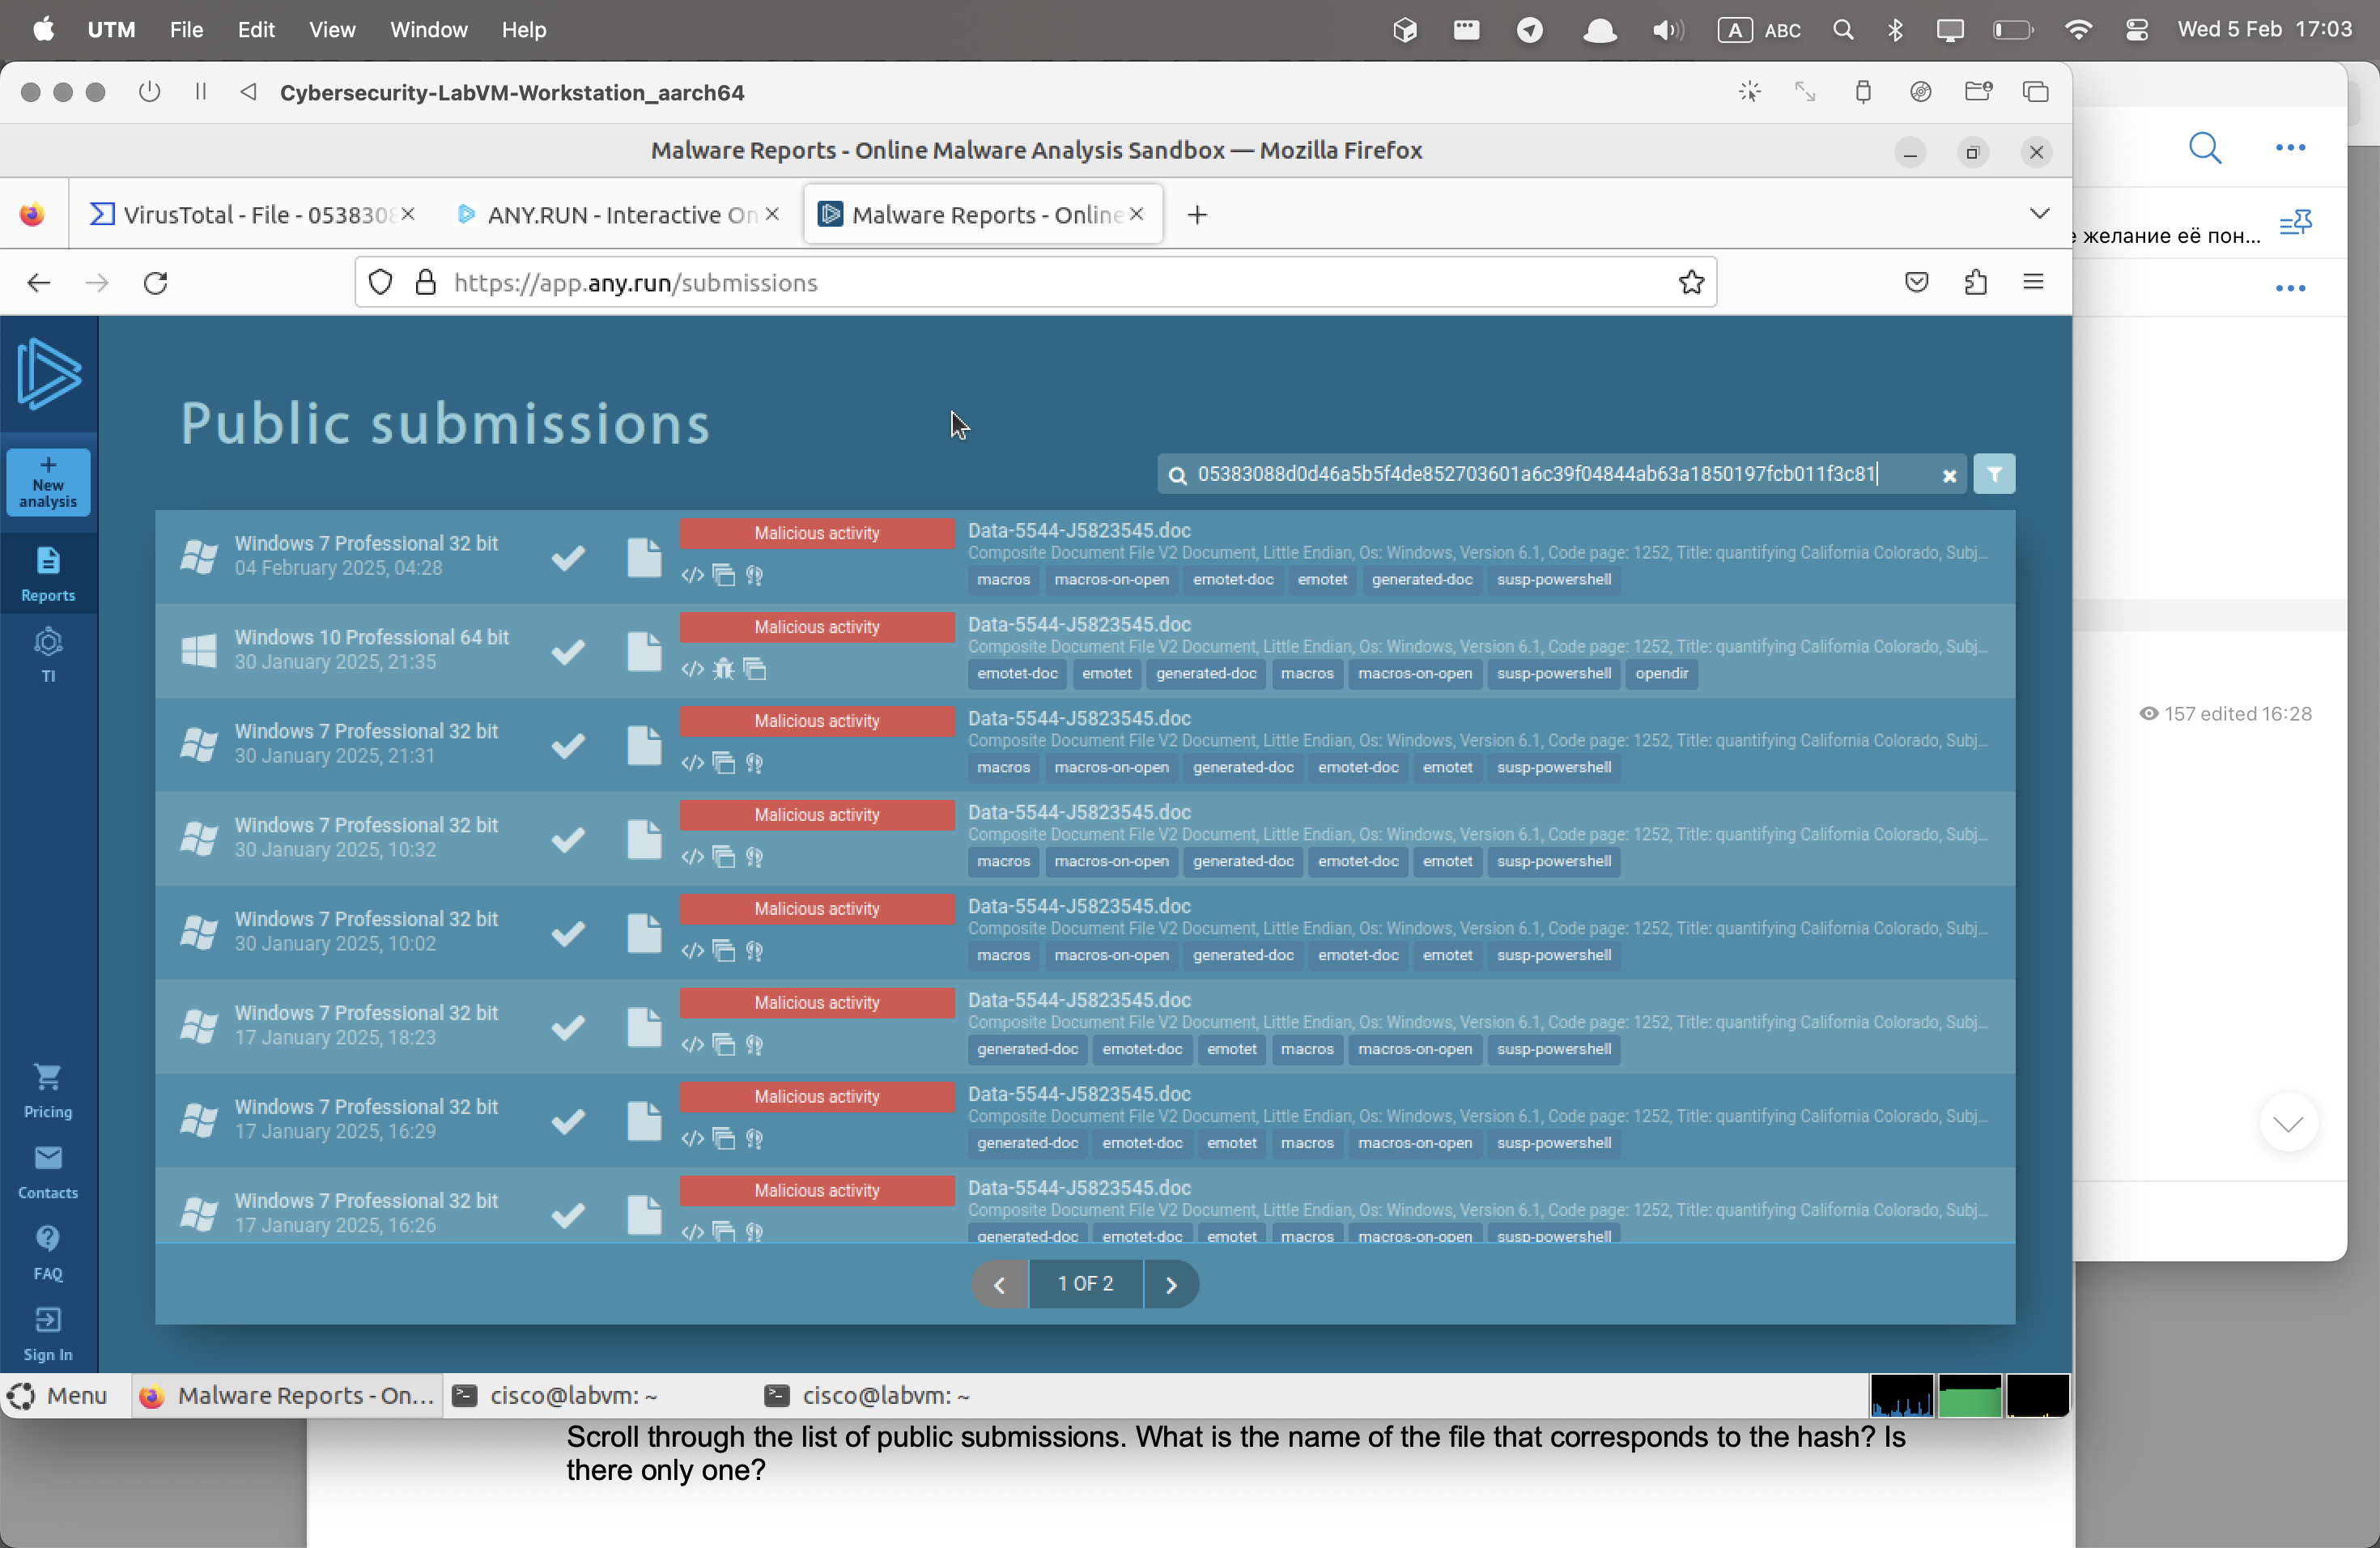
\includegraphics[width=1\textwidth]{7.png}

\subsection*{Step 2: Submit the IOC and review results}

\textbf{\colorbox{yellow}{Question 1: }} Scroll through the list of public submissions. What is the name of the file that corresponds to the hash? Is there only one? \\
\textbf{Answer: } The name of the file is \textbf{Data-5544-J5823545.doc}. No there are also one file with name \textbf{DocX69688X4511225.doc}.

\vspace{1\baselineskip}


\includegraphics[width=1\textwidth]{8.png}

\subsection*{Step 3: Explore the interface}

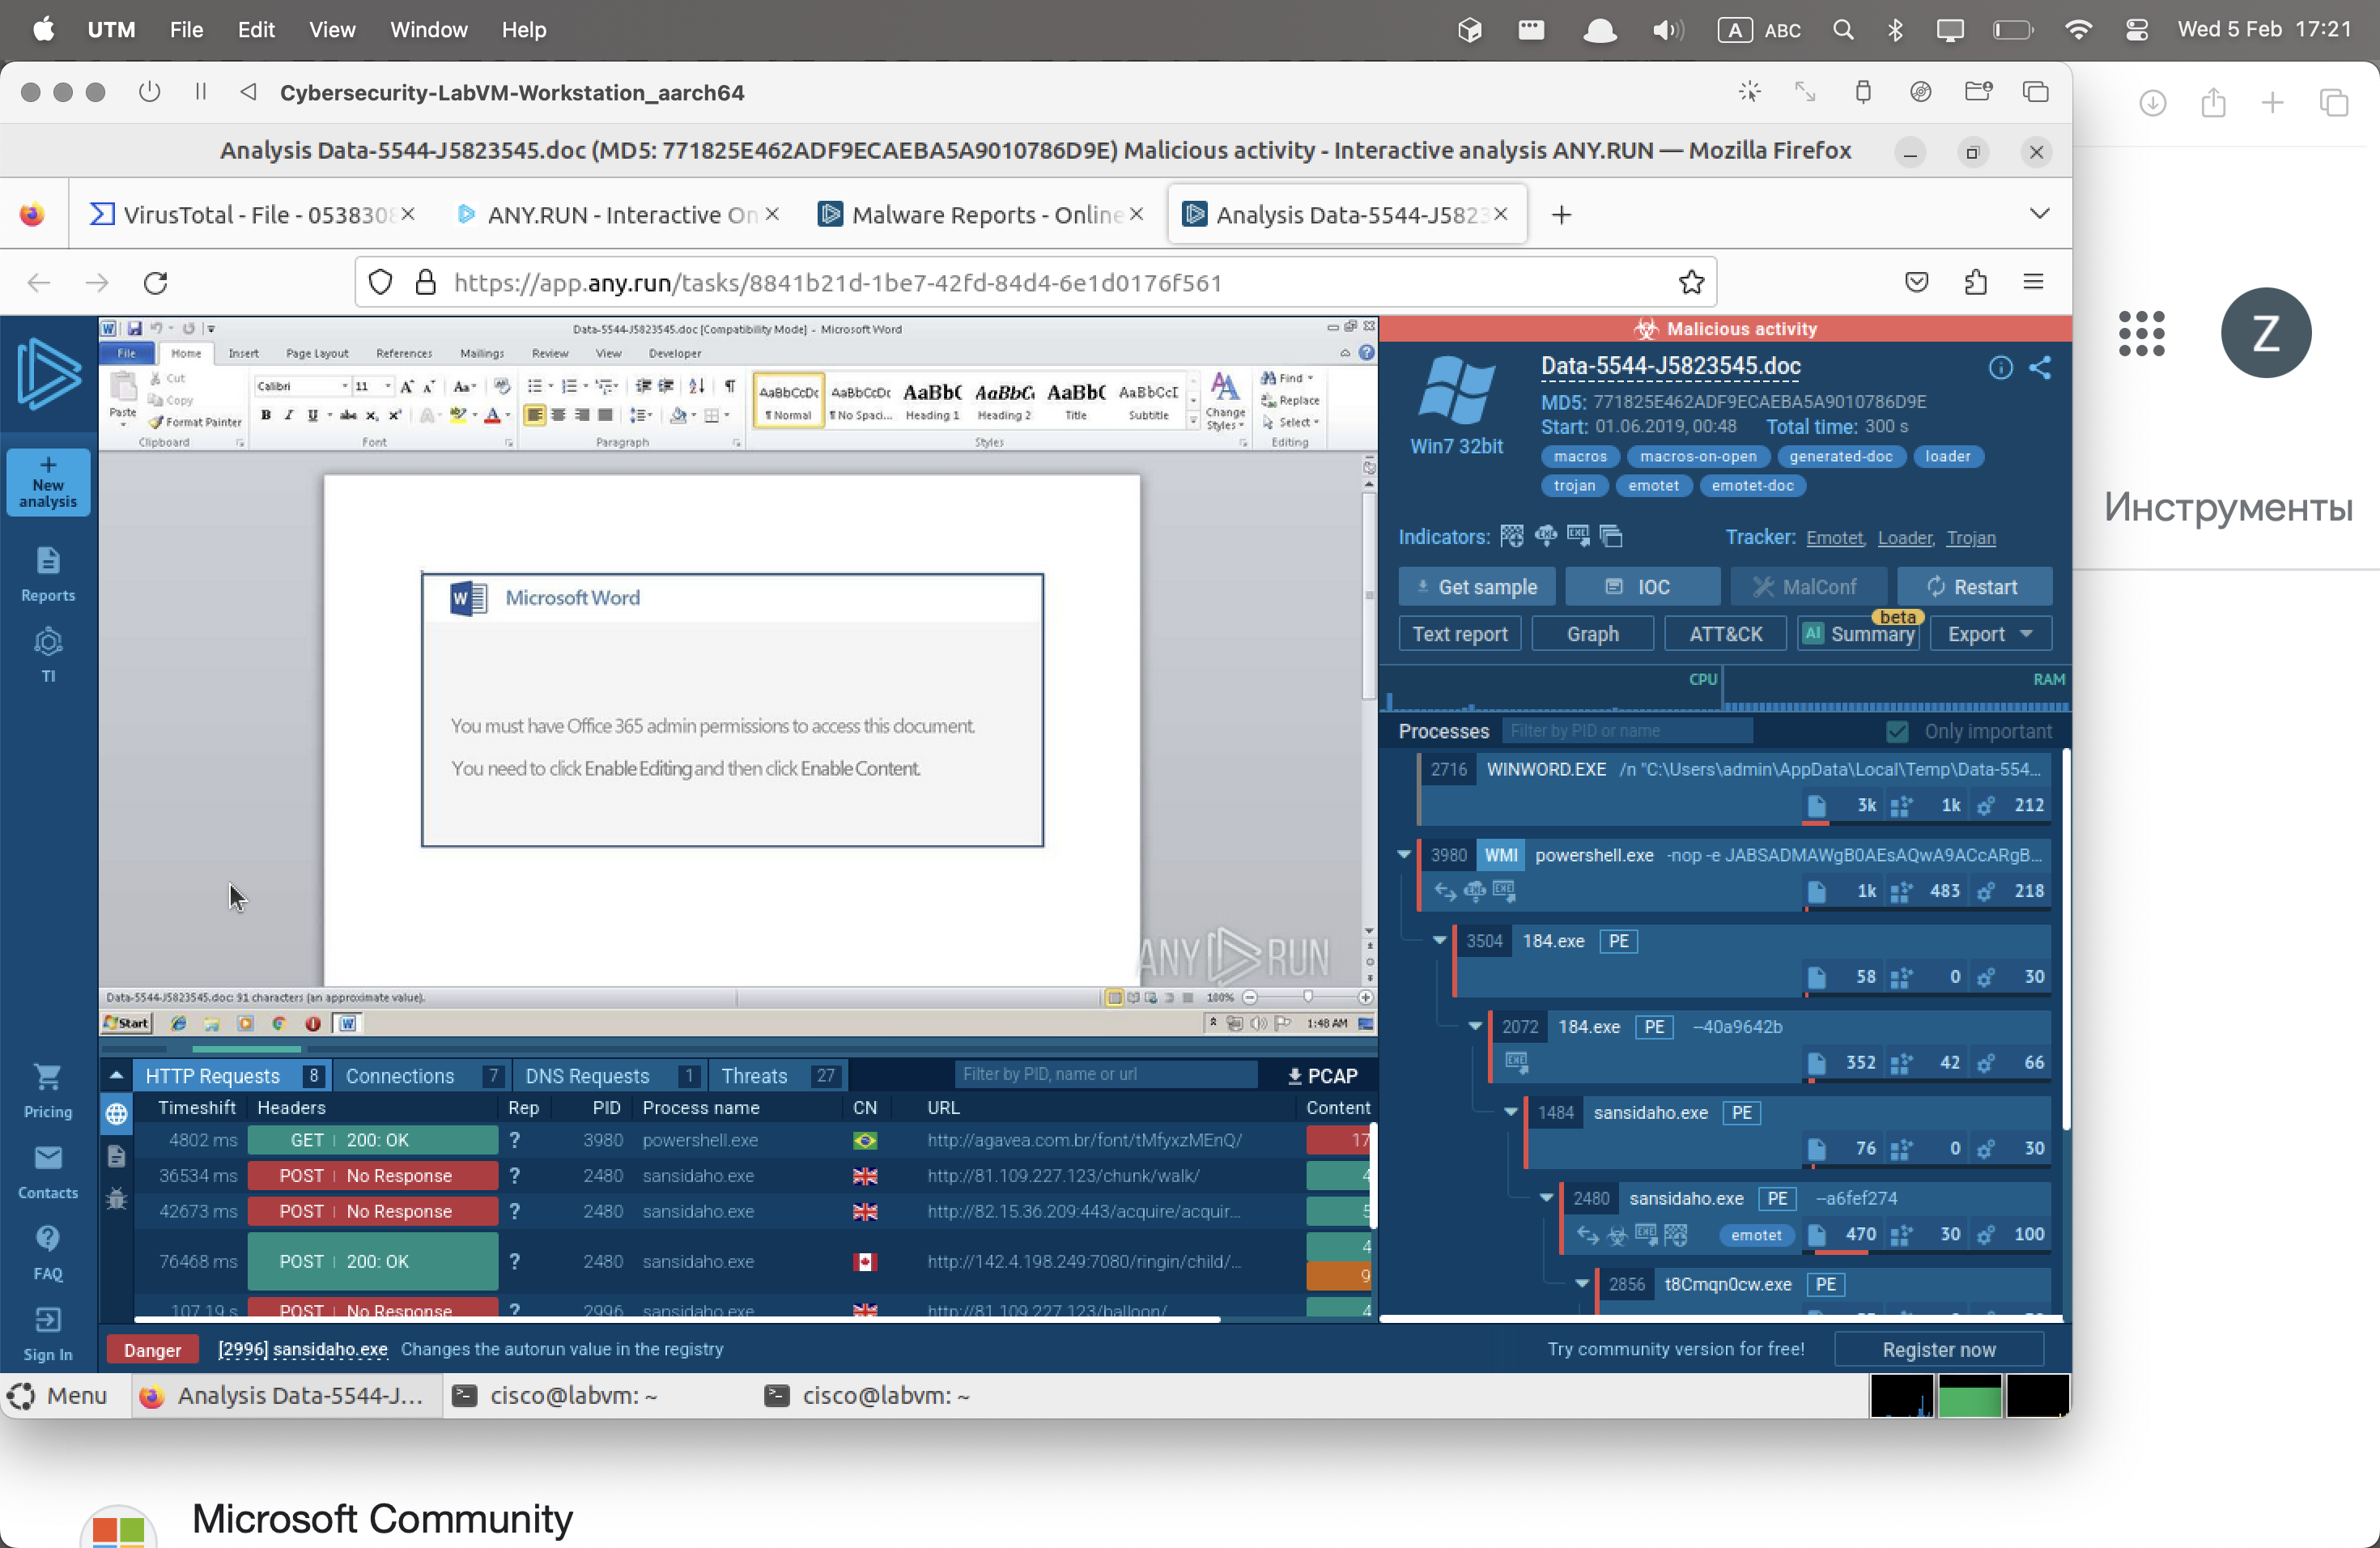
\includegraphics[width=1\textwidth]{9.png}

\textbf{\colorbox{yellow}{Question 2: }} Review the screens from start to finish. From what you see in the screens, what seems to be the first part of the virus infection process? \\
\textbf{Answer: } I think the first part of the virus was when the word asking enable content to start macros, in my opinion, exactly in this momemnt starting encoding of hash and running script. \\

\vspace{1\baselineskip}

\newpage

After this I clicked the first process and click to the more info to check what is first process

\vspace{1\baselineskip}

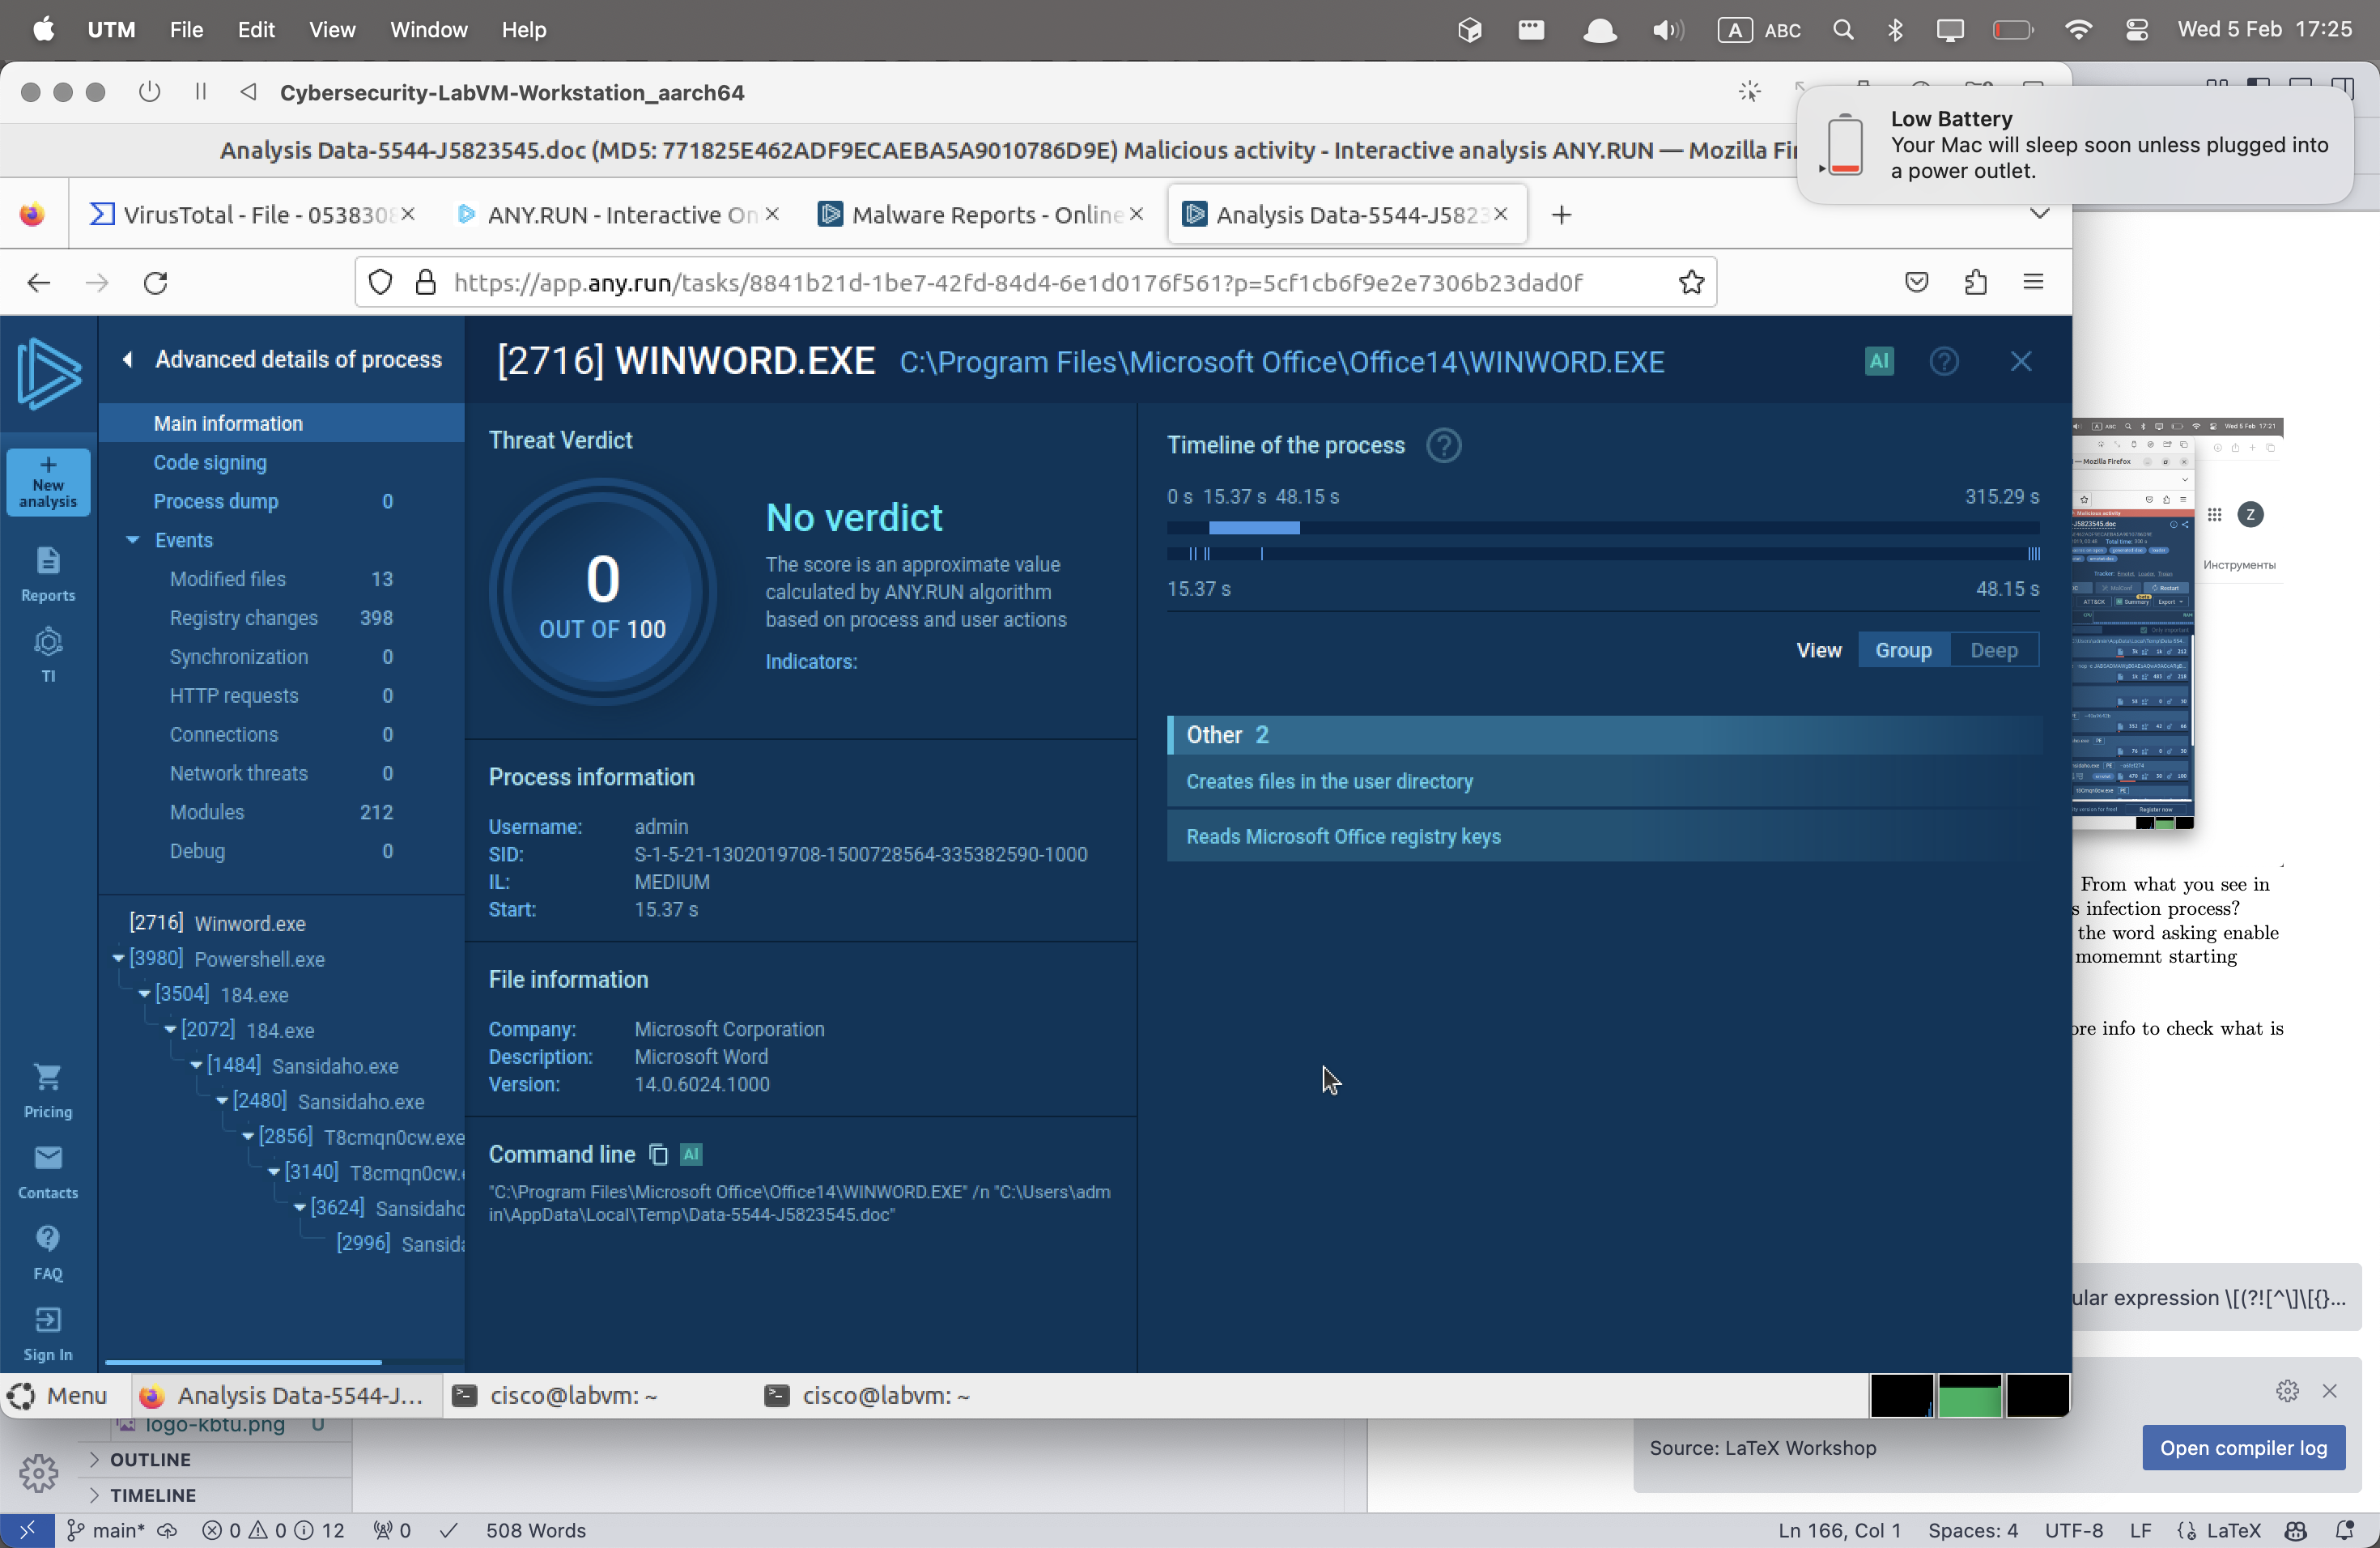
\includegraphics[width=1\textwidth]{10.png}

\vspace{1\baselineskip}

\textbf{\colorbox{yellow}{Question 3: }} Which process is this? \\
\textbf{Answer: } This is the process of Microsoft Word. \\

\vspace{1\baselineskip}

\textbf{\colorbox{yellow}{Question 4: }} Look at the command line. Which file was passed as an argument to the command that runs MS Word? \\
\textbf{Answer: } The file that was passed as an argument to the command that runs MS Word is \textbf{Data-5544-J5823545.doc}. \\

\vspace{1\baselineskip}

\textbf{\colorbox{yellow}{Question 5: }} What role do you think this document file played in the malware exploit? Feel free to search the web for your answer. \\
\textbf{Answer: } This document file played a role in the malware exploit by containing malicious macros that, when enabled, executed a script that encoded the hash and ran the script. This allowed the malware to execute and infect the system. \\

\newpage

\subsection*{Step 4: Analyze an Obfuscated Script}

I clicked the next one process and checked.

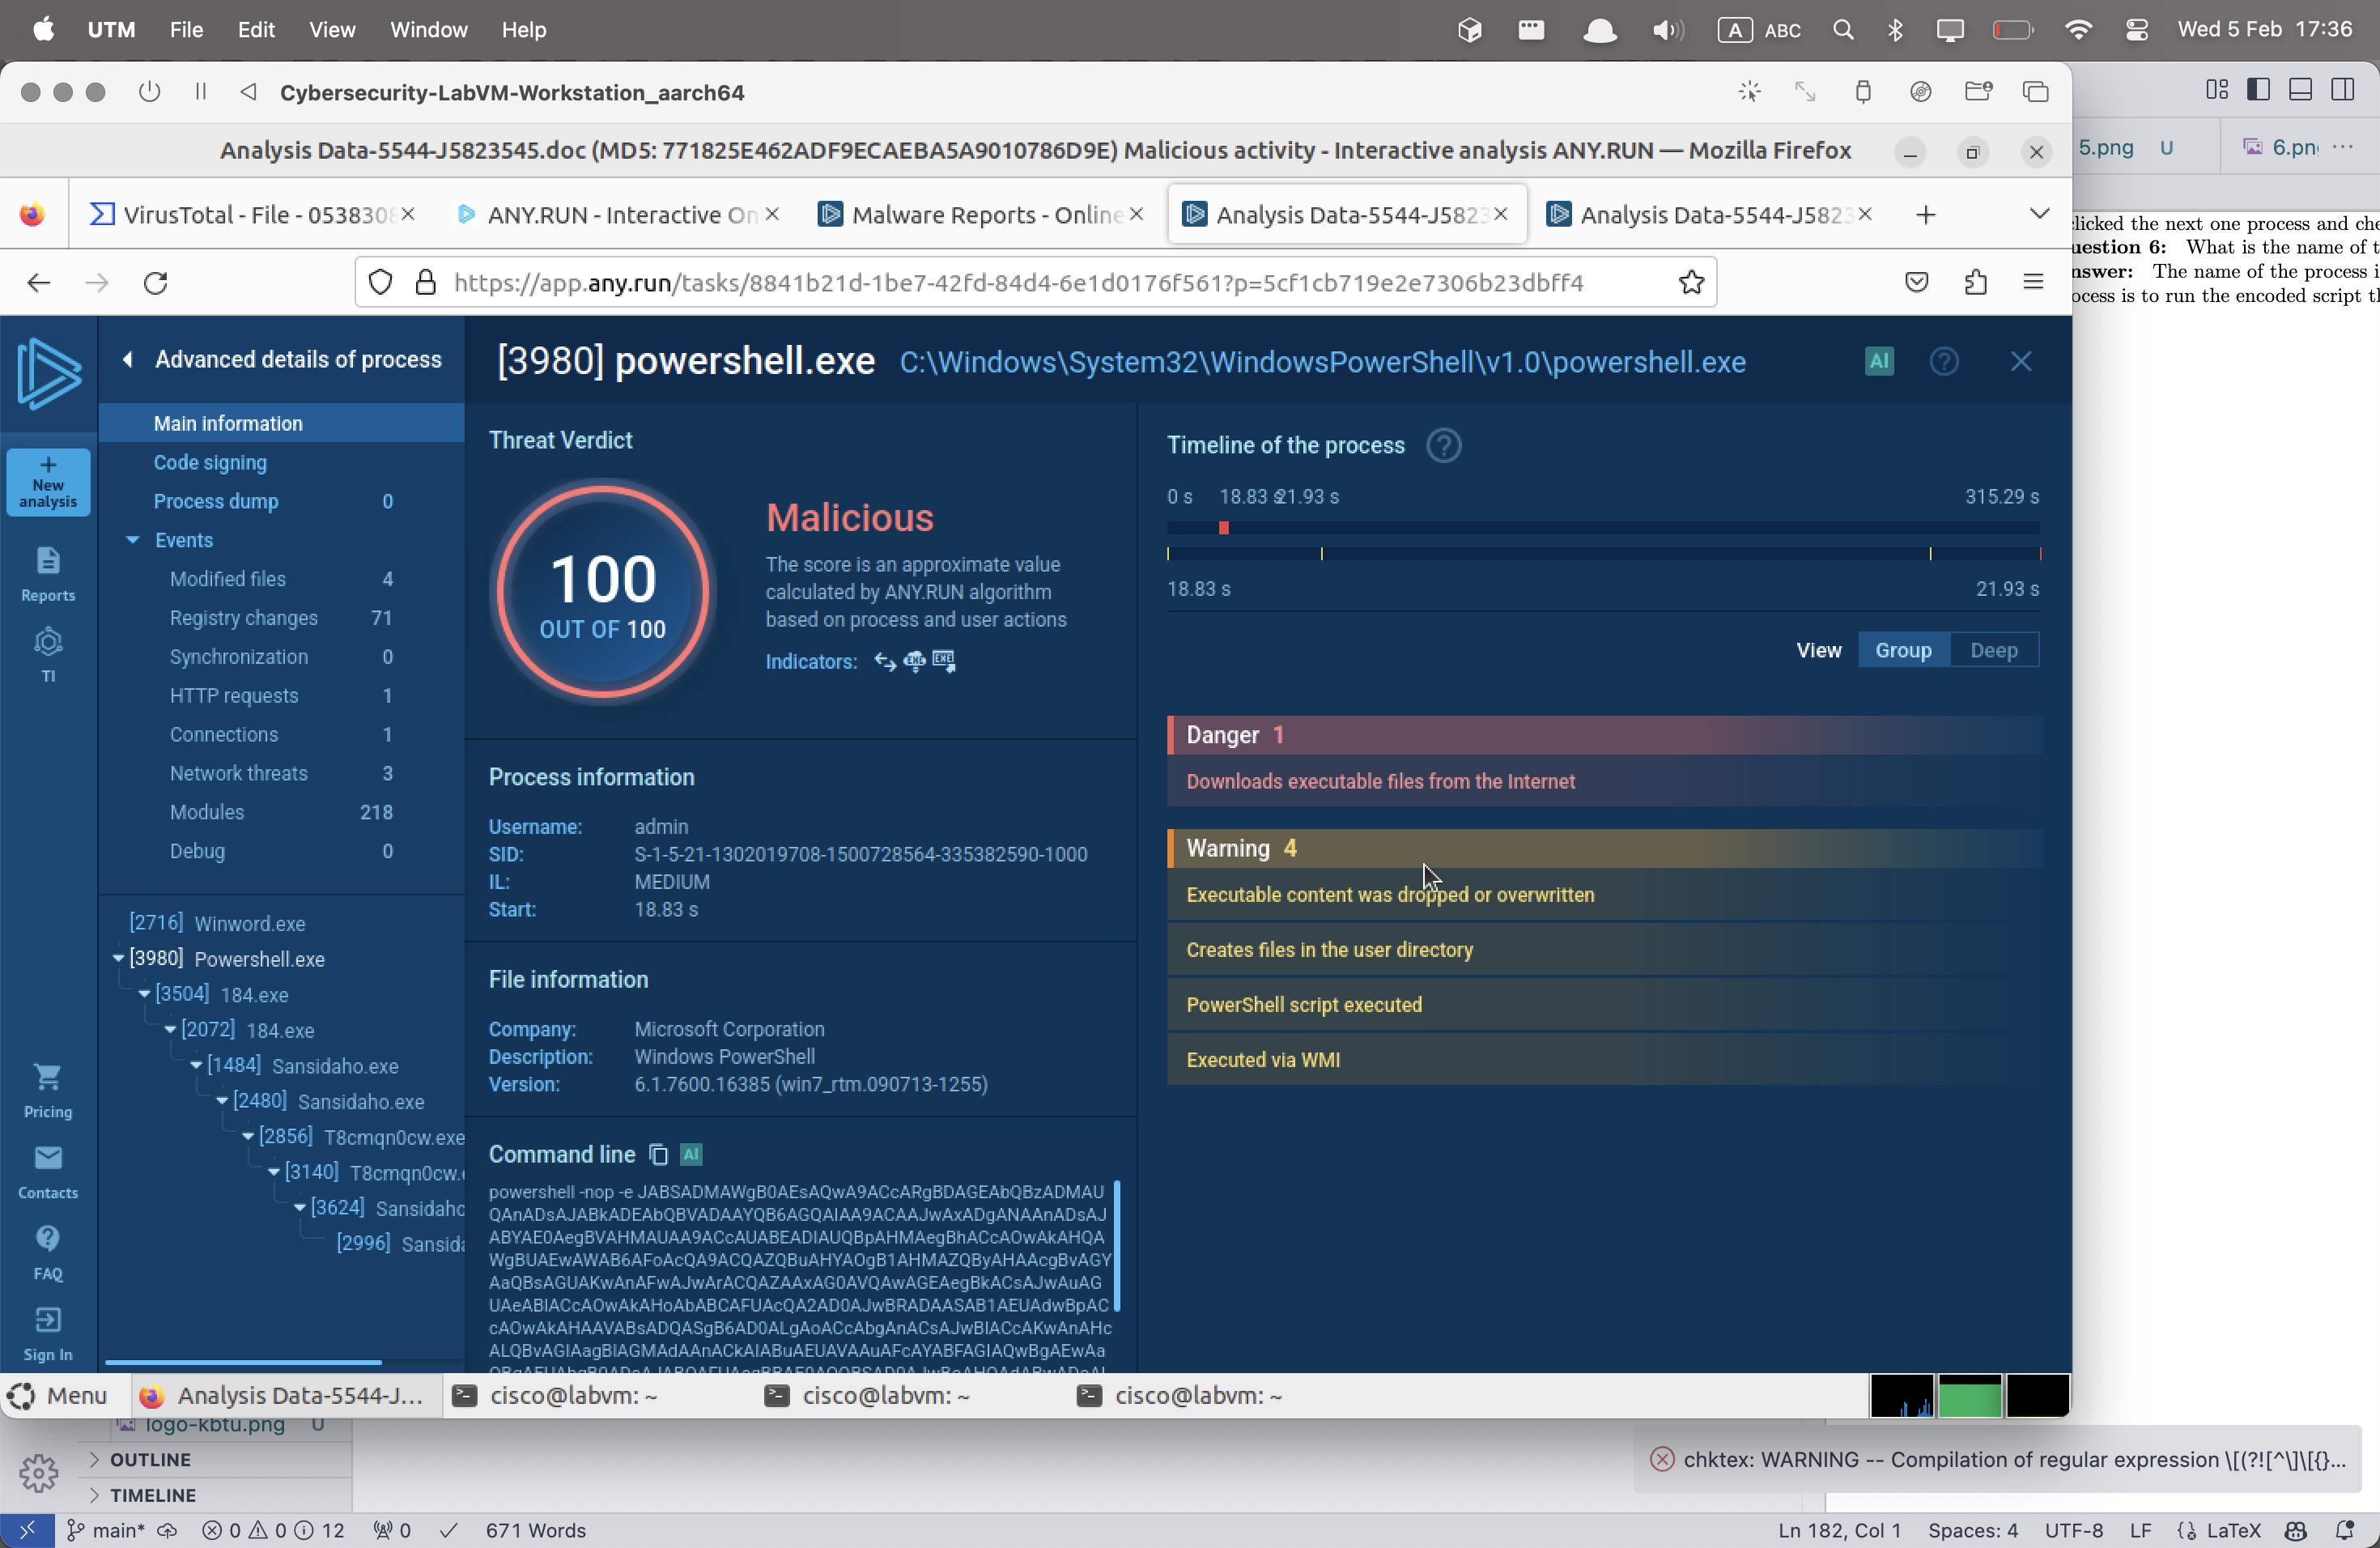
\includegraphics[width=1\textwidth]{11.png}

\textbf{\colorbox{yellow}{Question 6: }} What is the name of the process? What is its purpose? \\
\textbf{Answer: } The name of the process is \textbf{powershell.exe}. The purpose of this process is to run the encoded script that was extracted from the document file. \\

\vspace{1\baselineskip}

\textbf{\colorbox{yellow}{Question 7: }} PowerShell is often used by threat actors in living-off-the-land (LotL) attacks. What is an LotL attack, and how does PowerShell enable these attacks? Use the internet to search for answers as needed.  \\

\textbf{Answer: } Living-off-the-land (LotL) attacks are attacks that use legitimate tools and processes that are already present on a system to carry out malicious activities. PowerShell enables these attacks by allowing threat actors to run scripts and commands that can be used to download and execute. \\

\vspace{1\baselineskip}

\newpage

After that step by step I input command to the file using cat command and after that cut the powershell -nop -e, to left only hash.

\vspace{1\baselineskip}

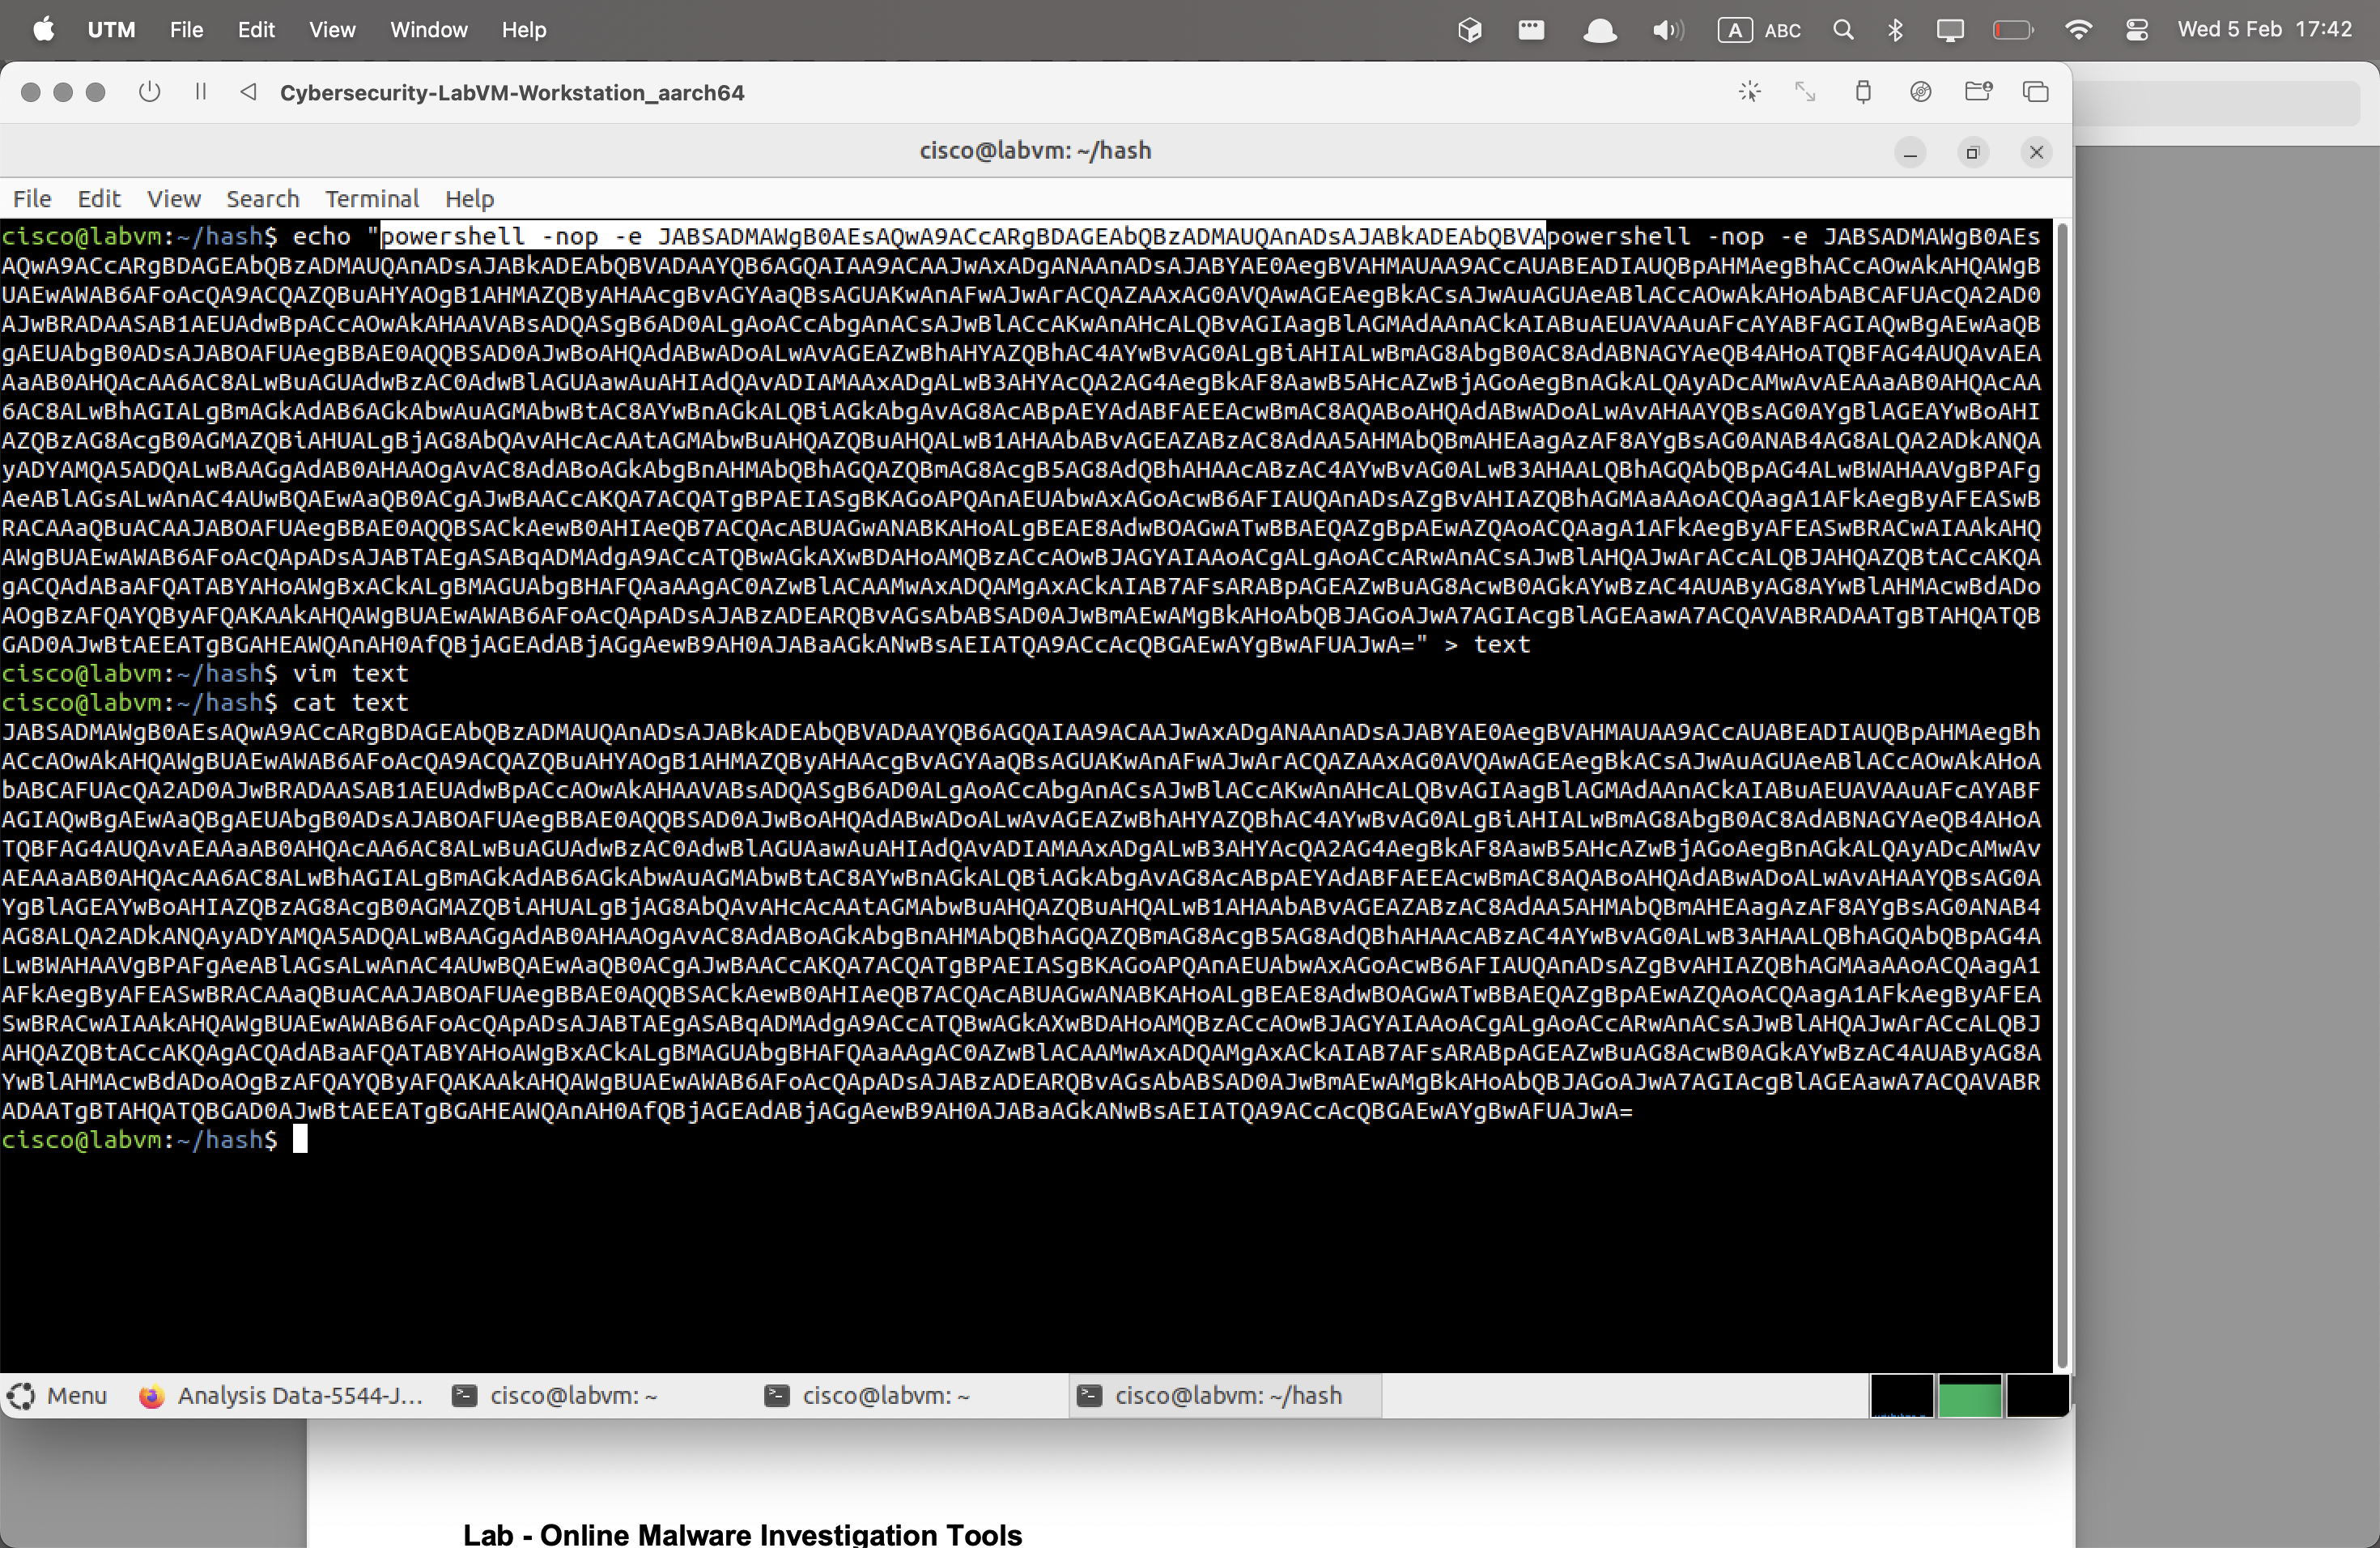
\includegraphics[width=1\textwidth]{12.png}

\vspace{1\baselineskip}

I encoded the hash and get this bash-script.

\vspace{1\baselineskip}

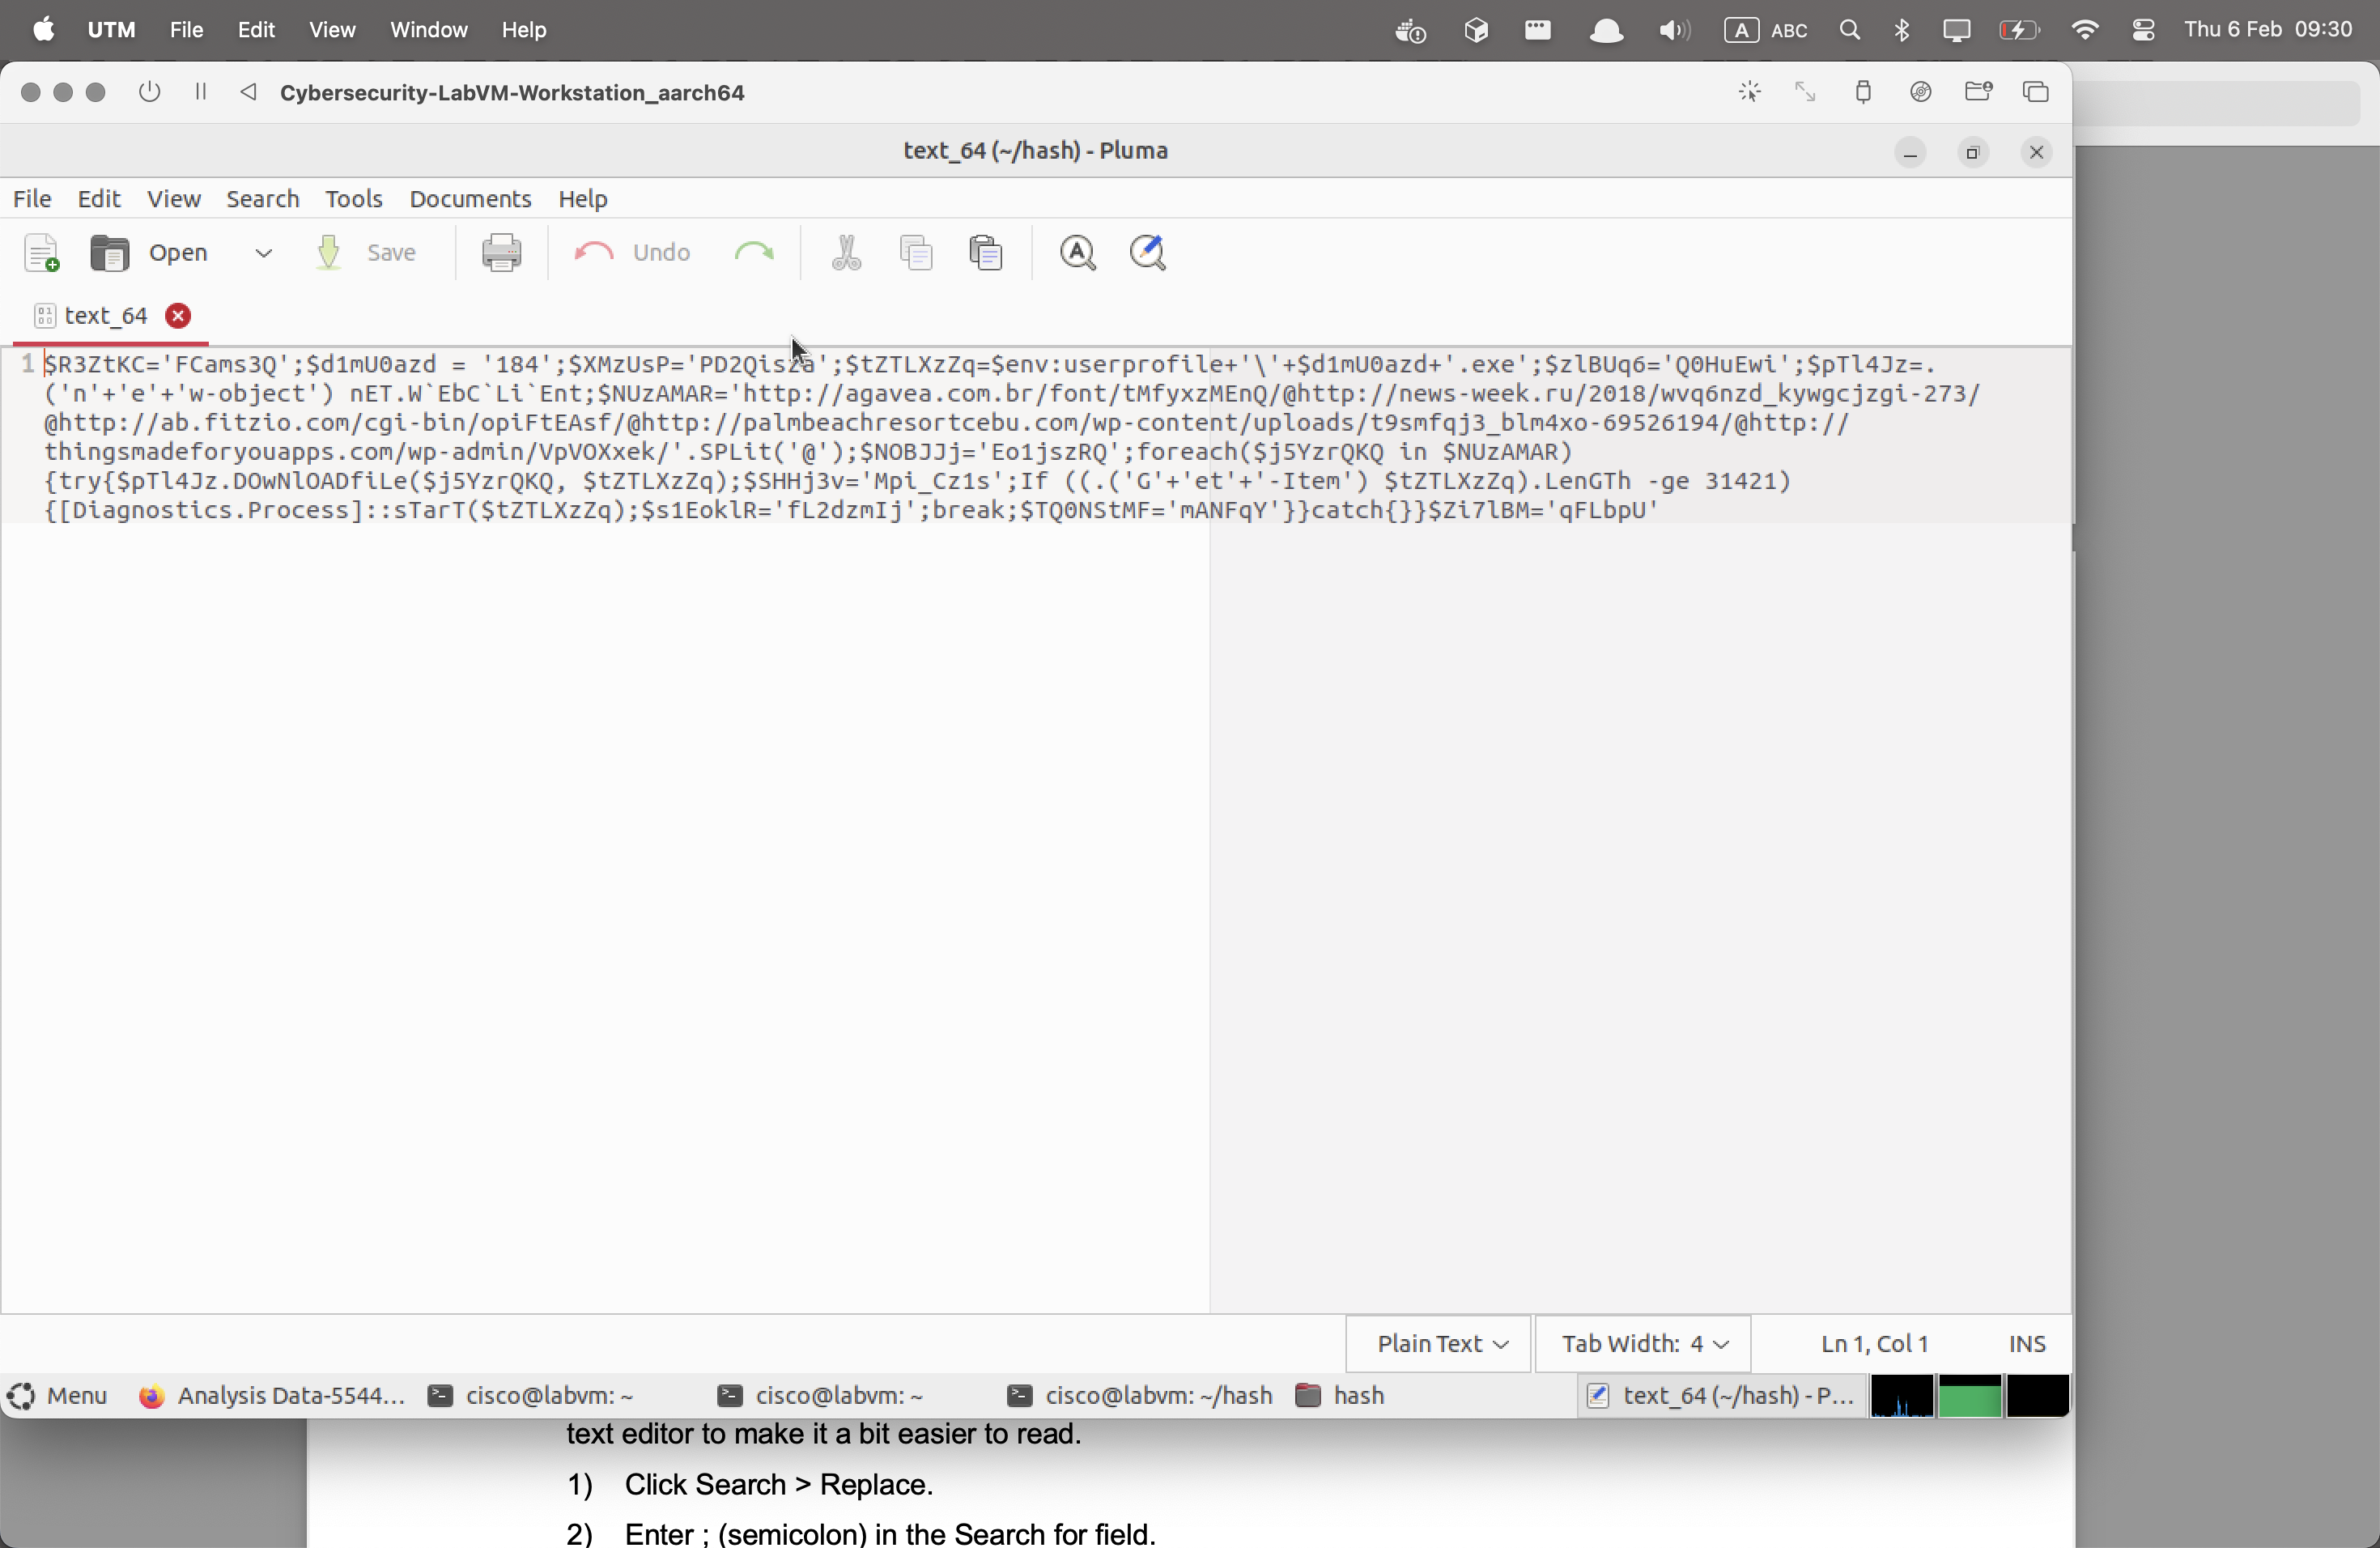
\includegraphics[width=1\textwidth]{13.png}

\newpage

How was said in the steps I formatted the script to make it more readable and get this script.

\vspace{1\baselineskip}

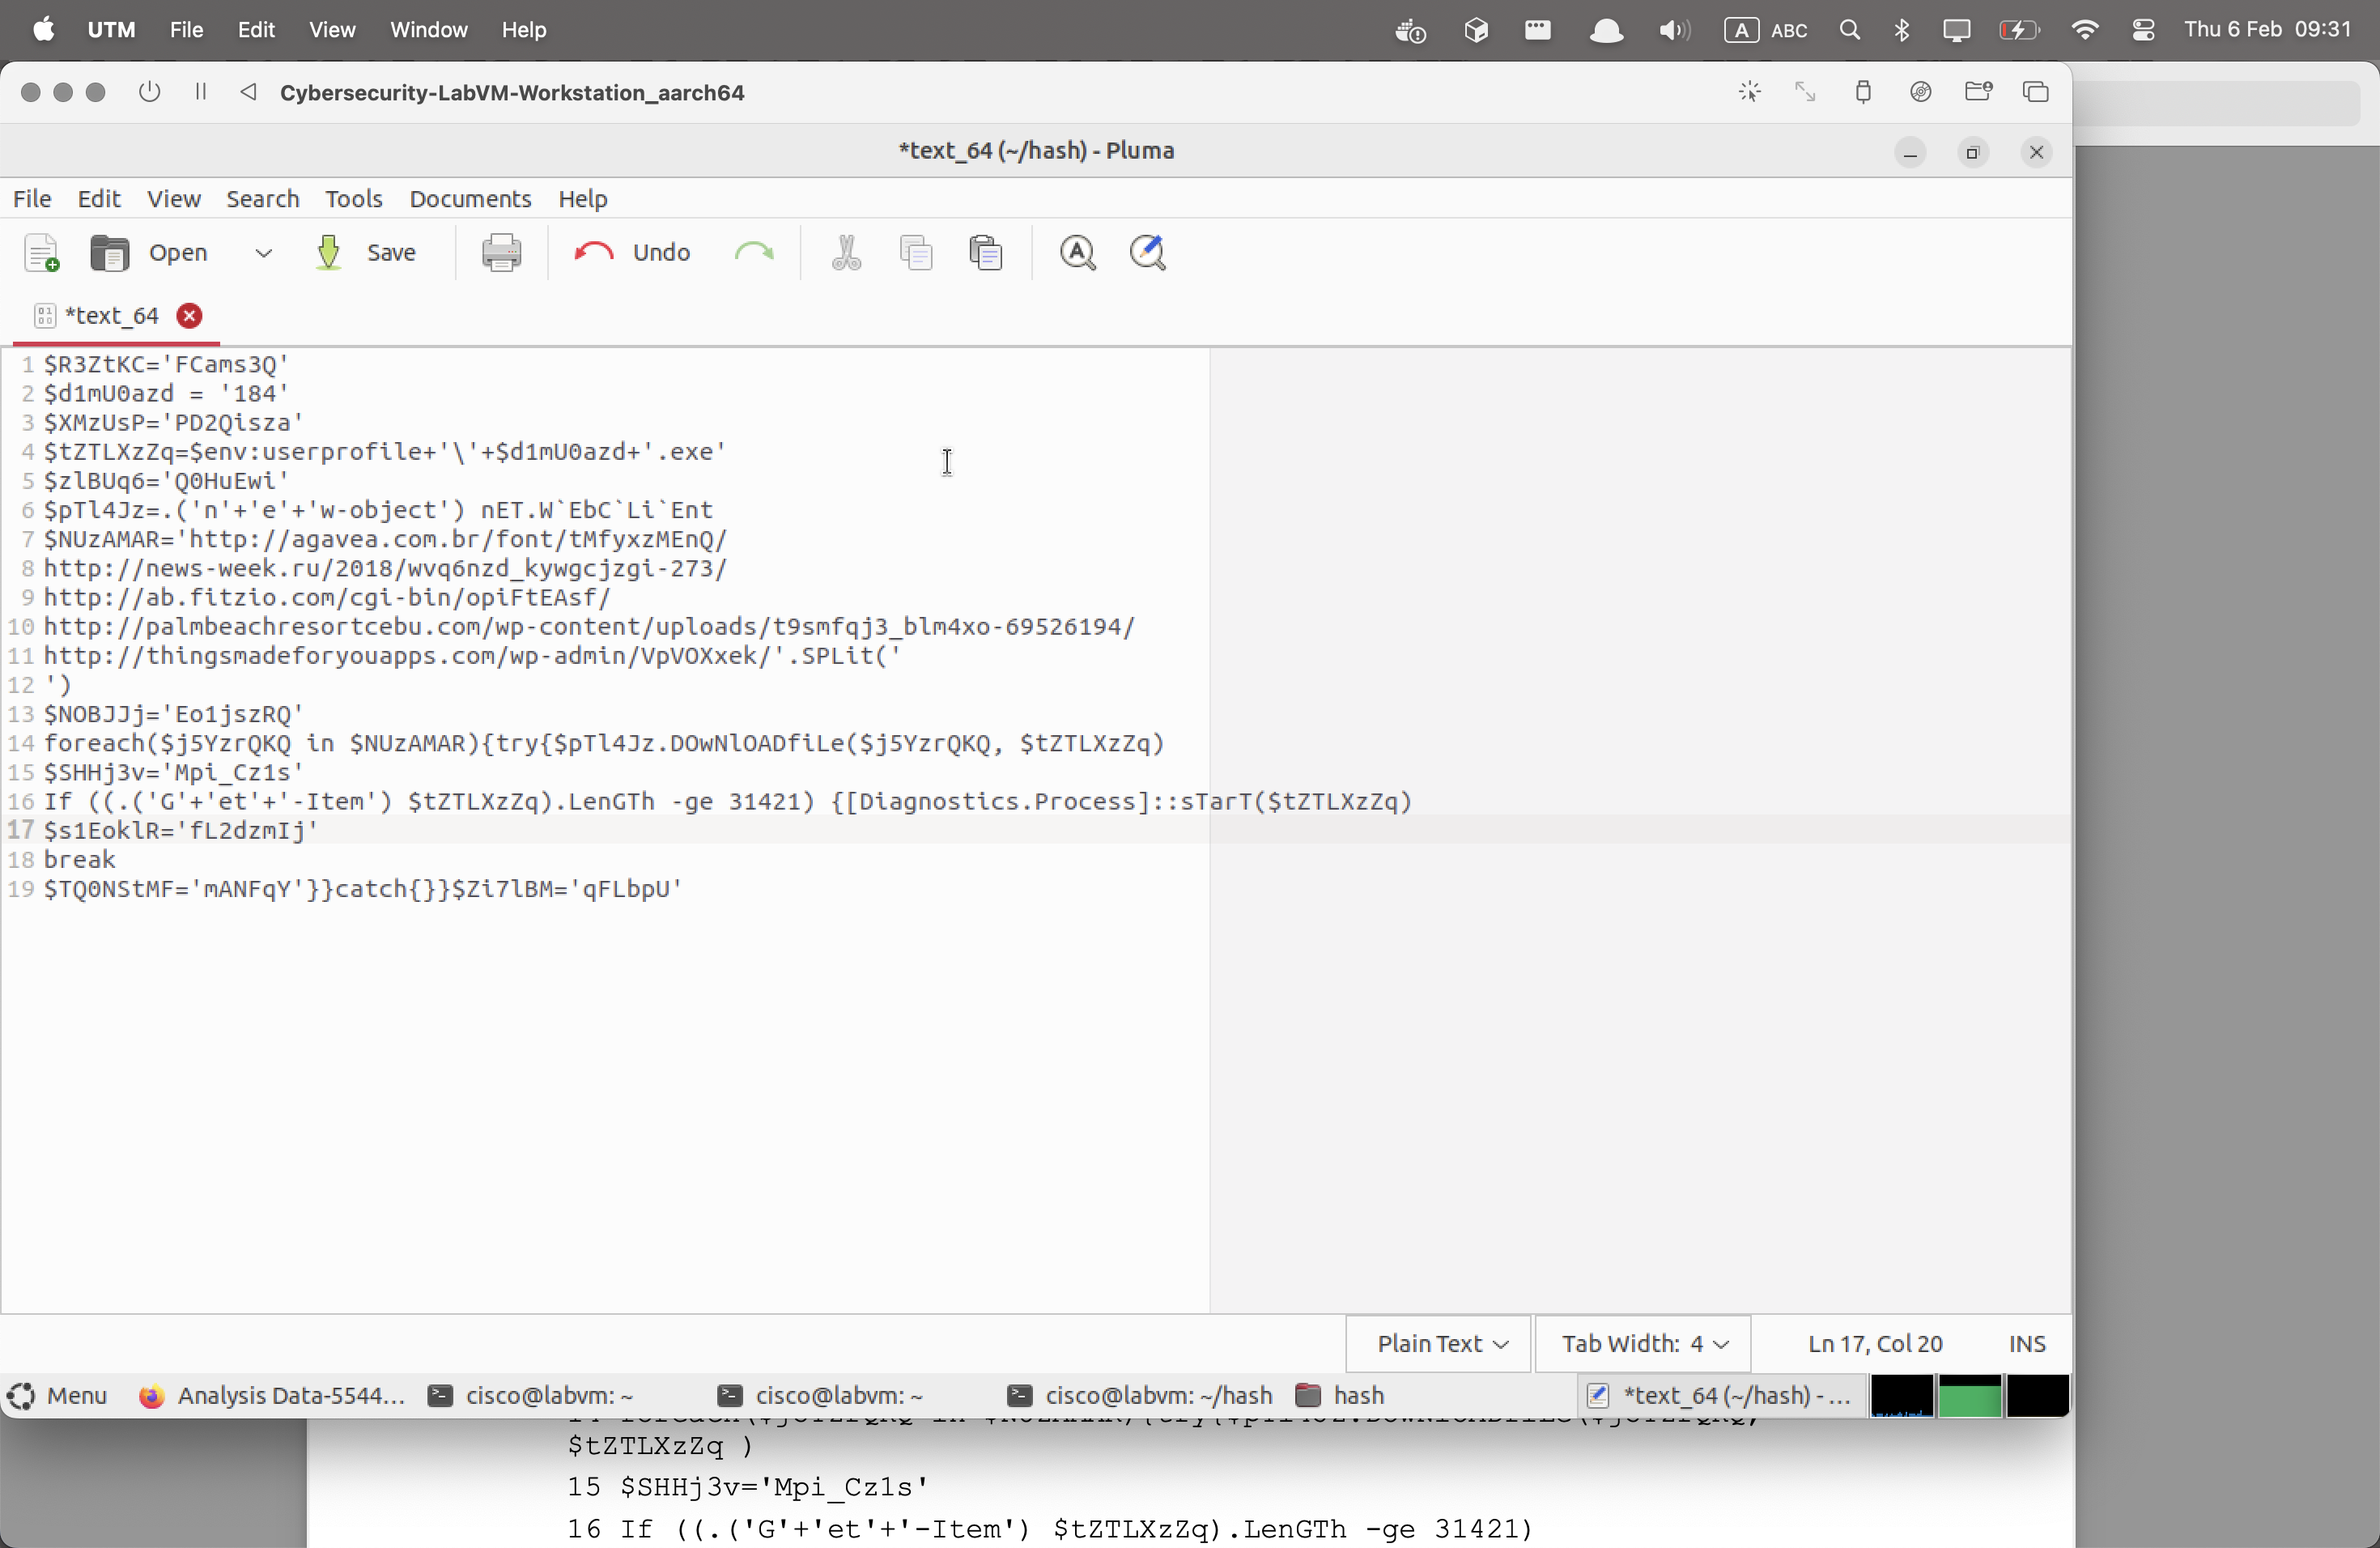
\includegraphics[width=1\textwidth]{14.png}

\vspace{1\baselineskip}

And saved to show in the future.

\vspace{1\baselineskip}

\newpage

\subsection*{Step 5: Interpret the Malware Script}

\subsubsection*{Notice that a series of URLs appear in the code. Submit several of them to ANY.RUN, VirusTotal, or
another service to see if they are malicious.}

I submitted the first URL (http://agavea.com.br/font/tMfyxzMEnQ) to the VirusTotal website and got this result.

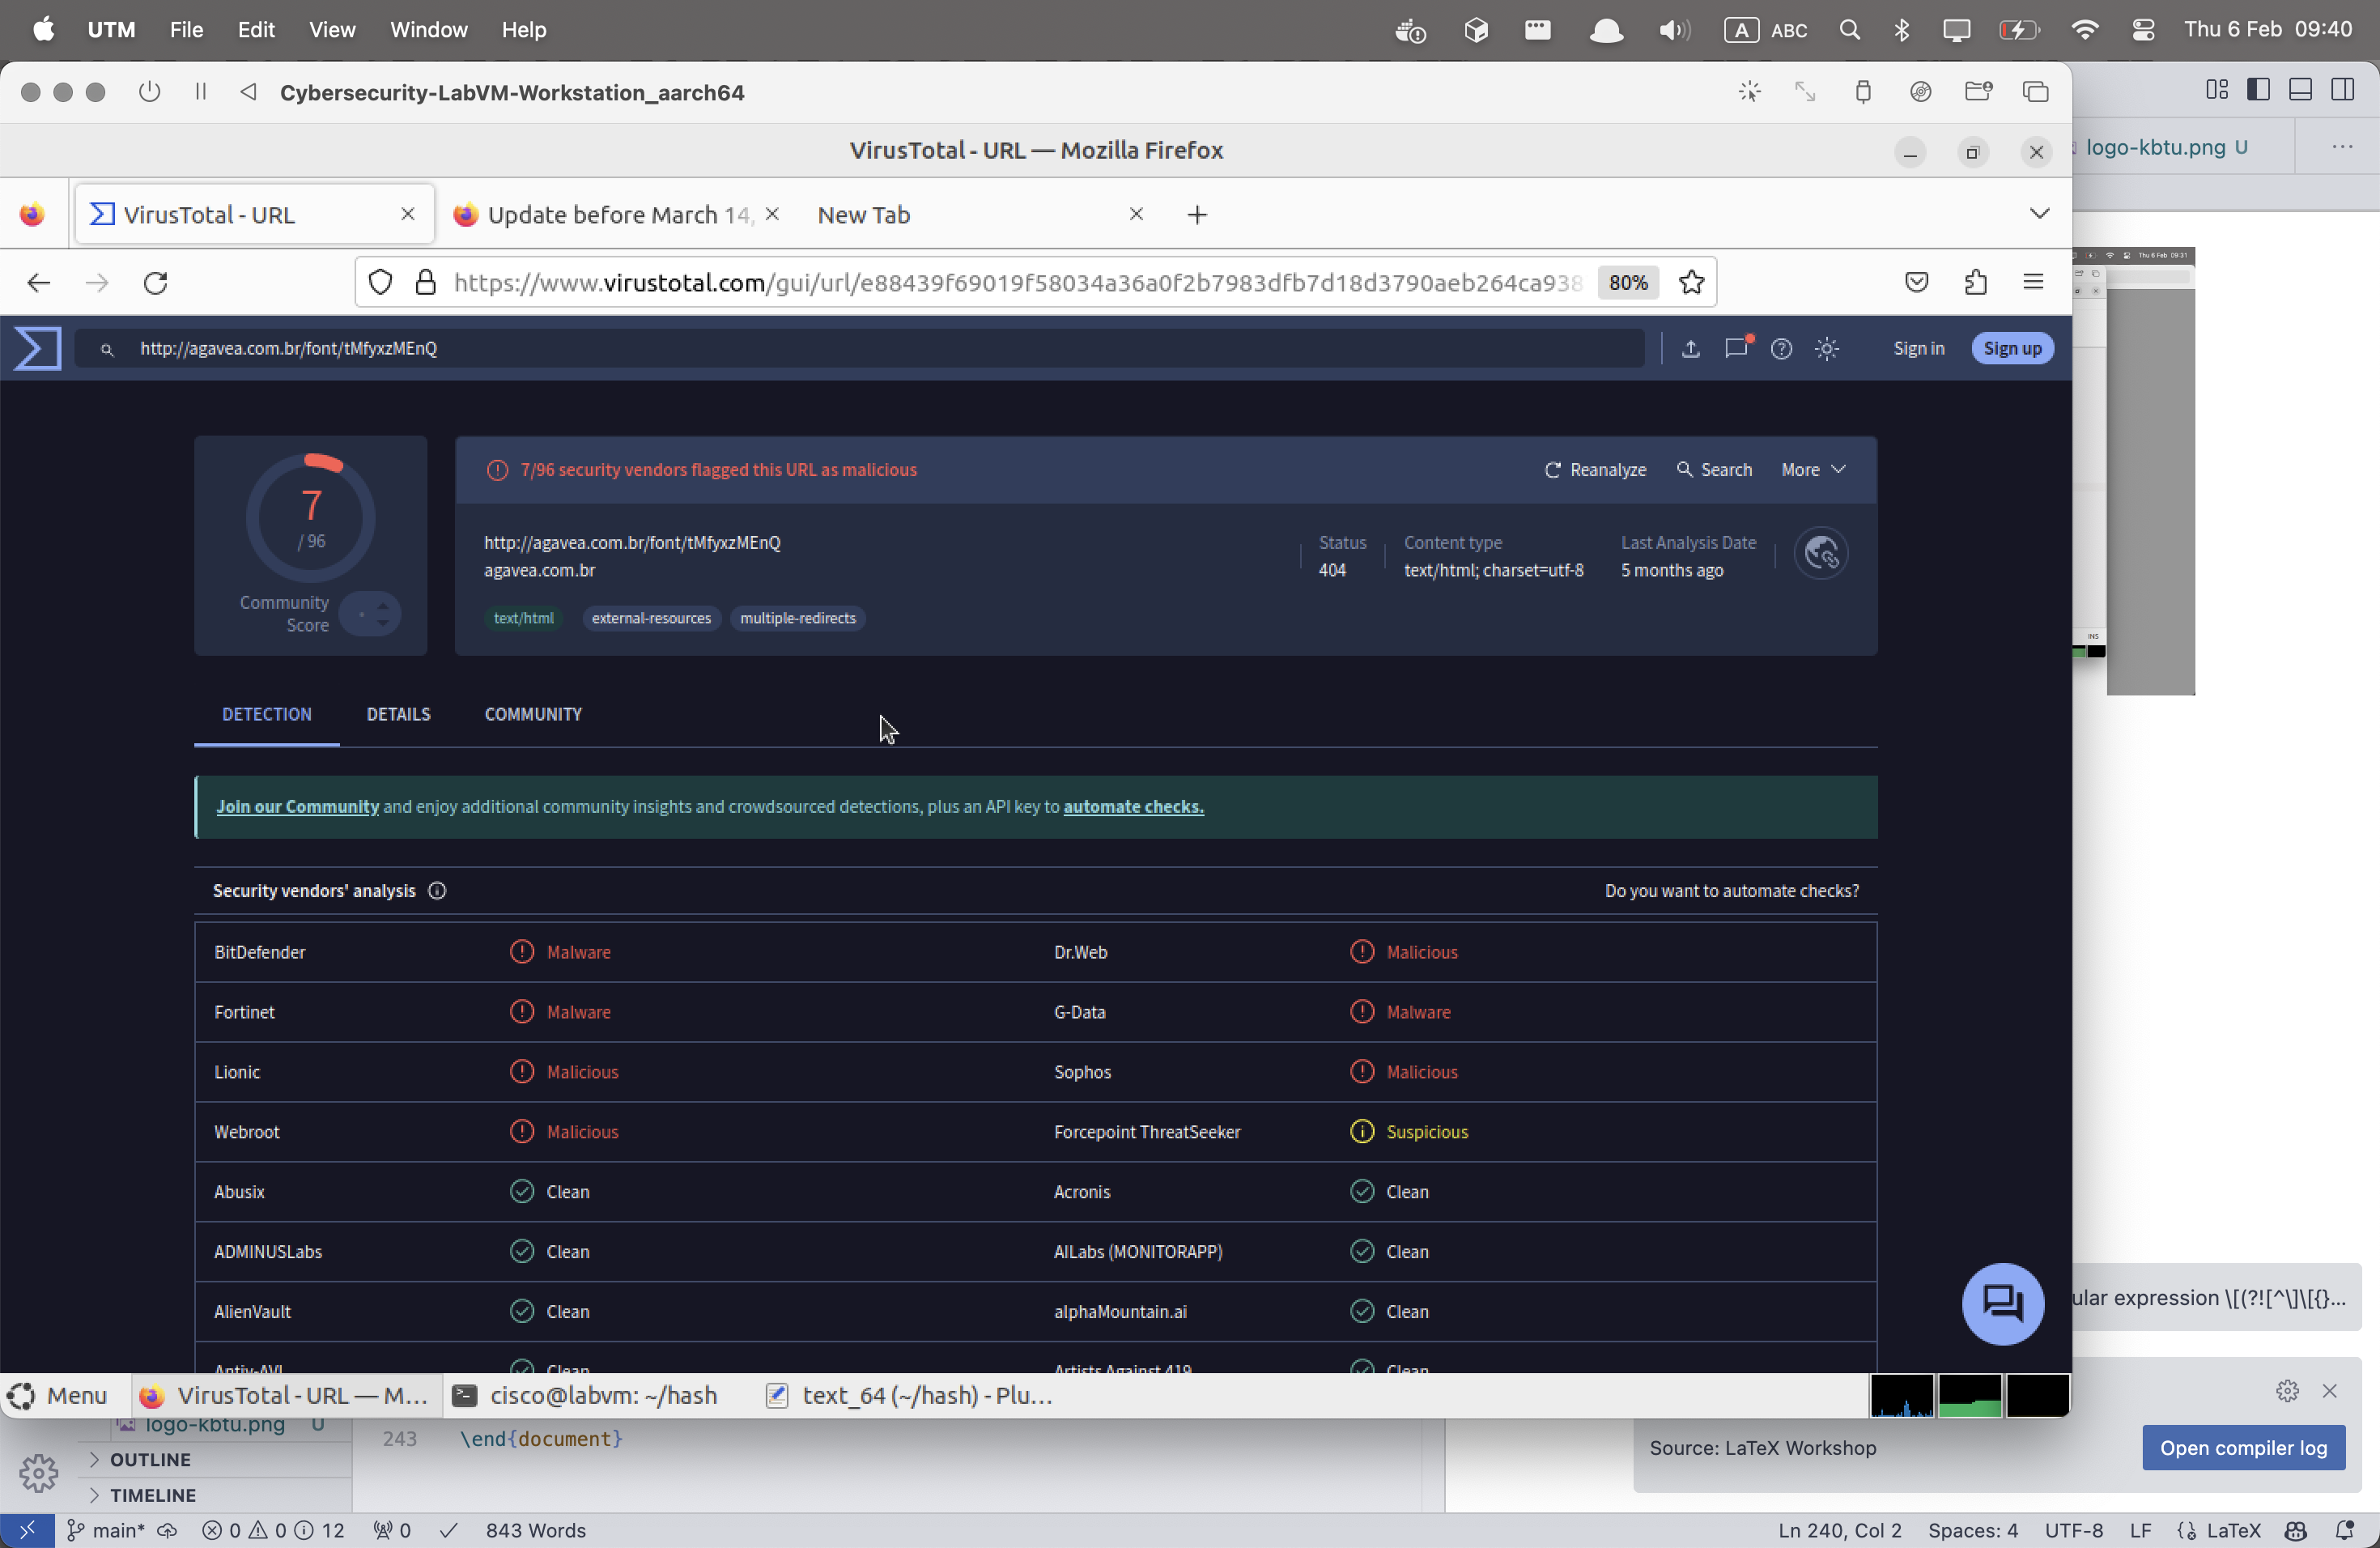
\includegraphics[width=0.9\textwidth]{15.png}

I submitted the second URL (http://ab.fitzio.com) to the VirusTotal website and got this result.

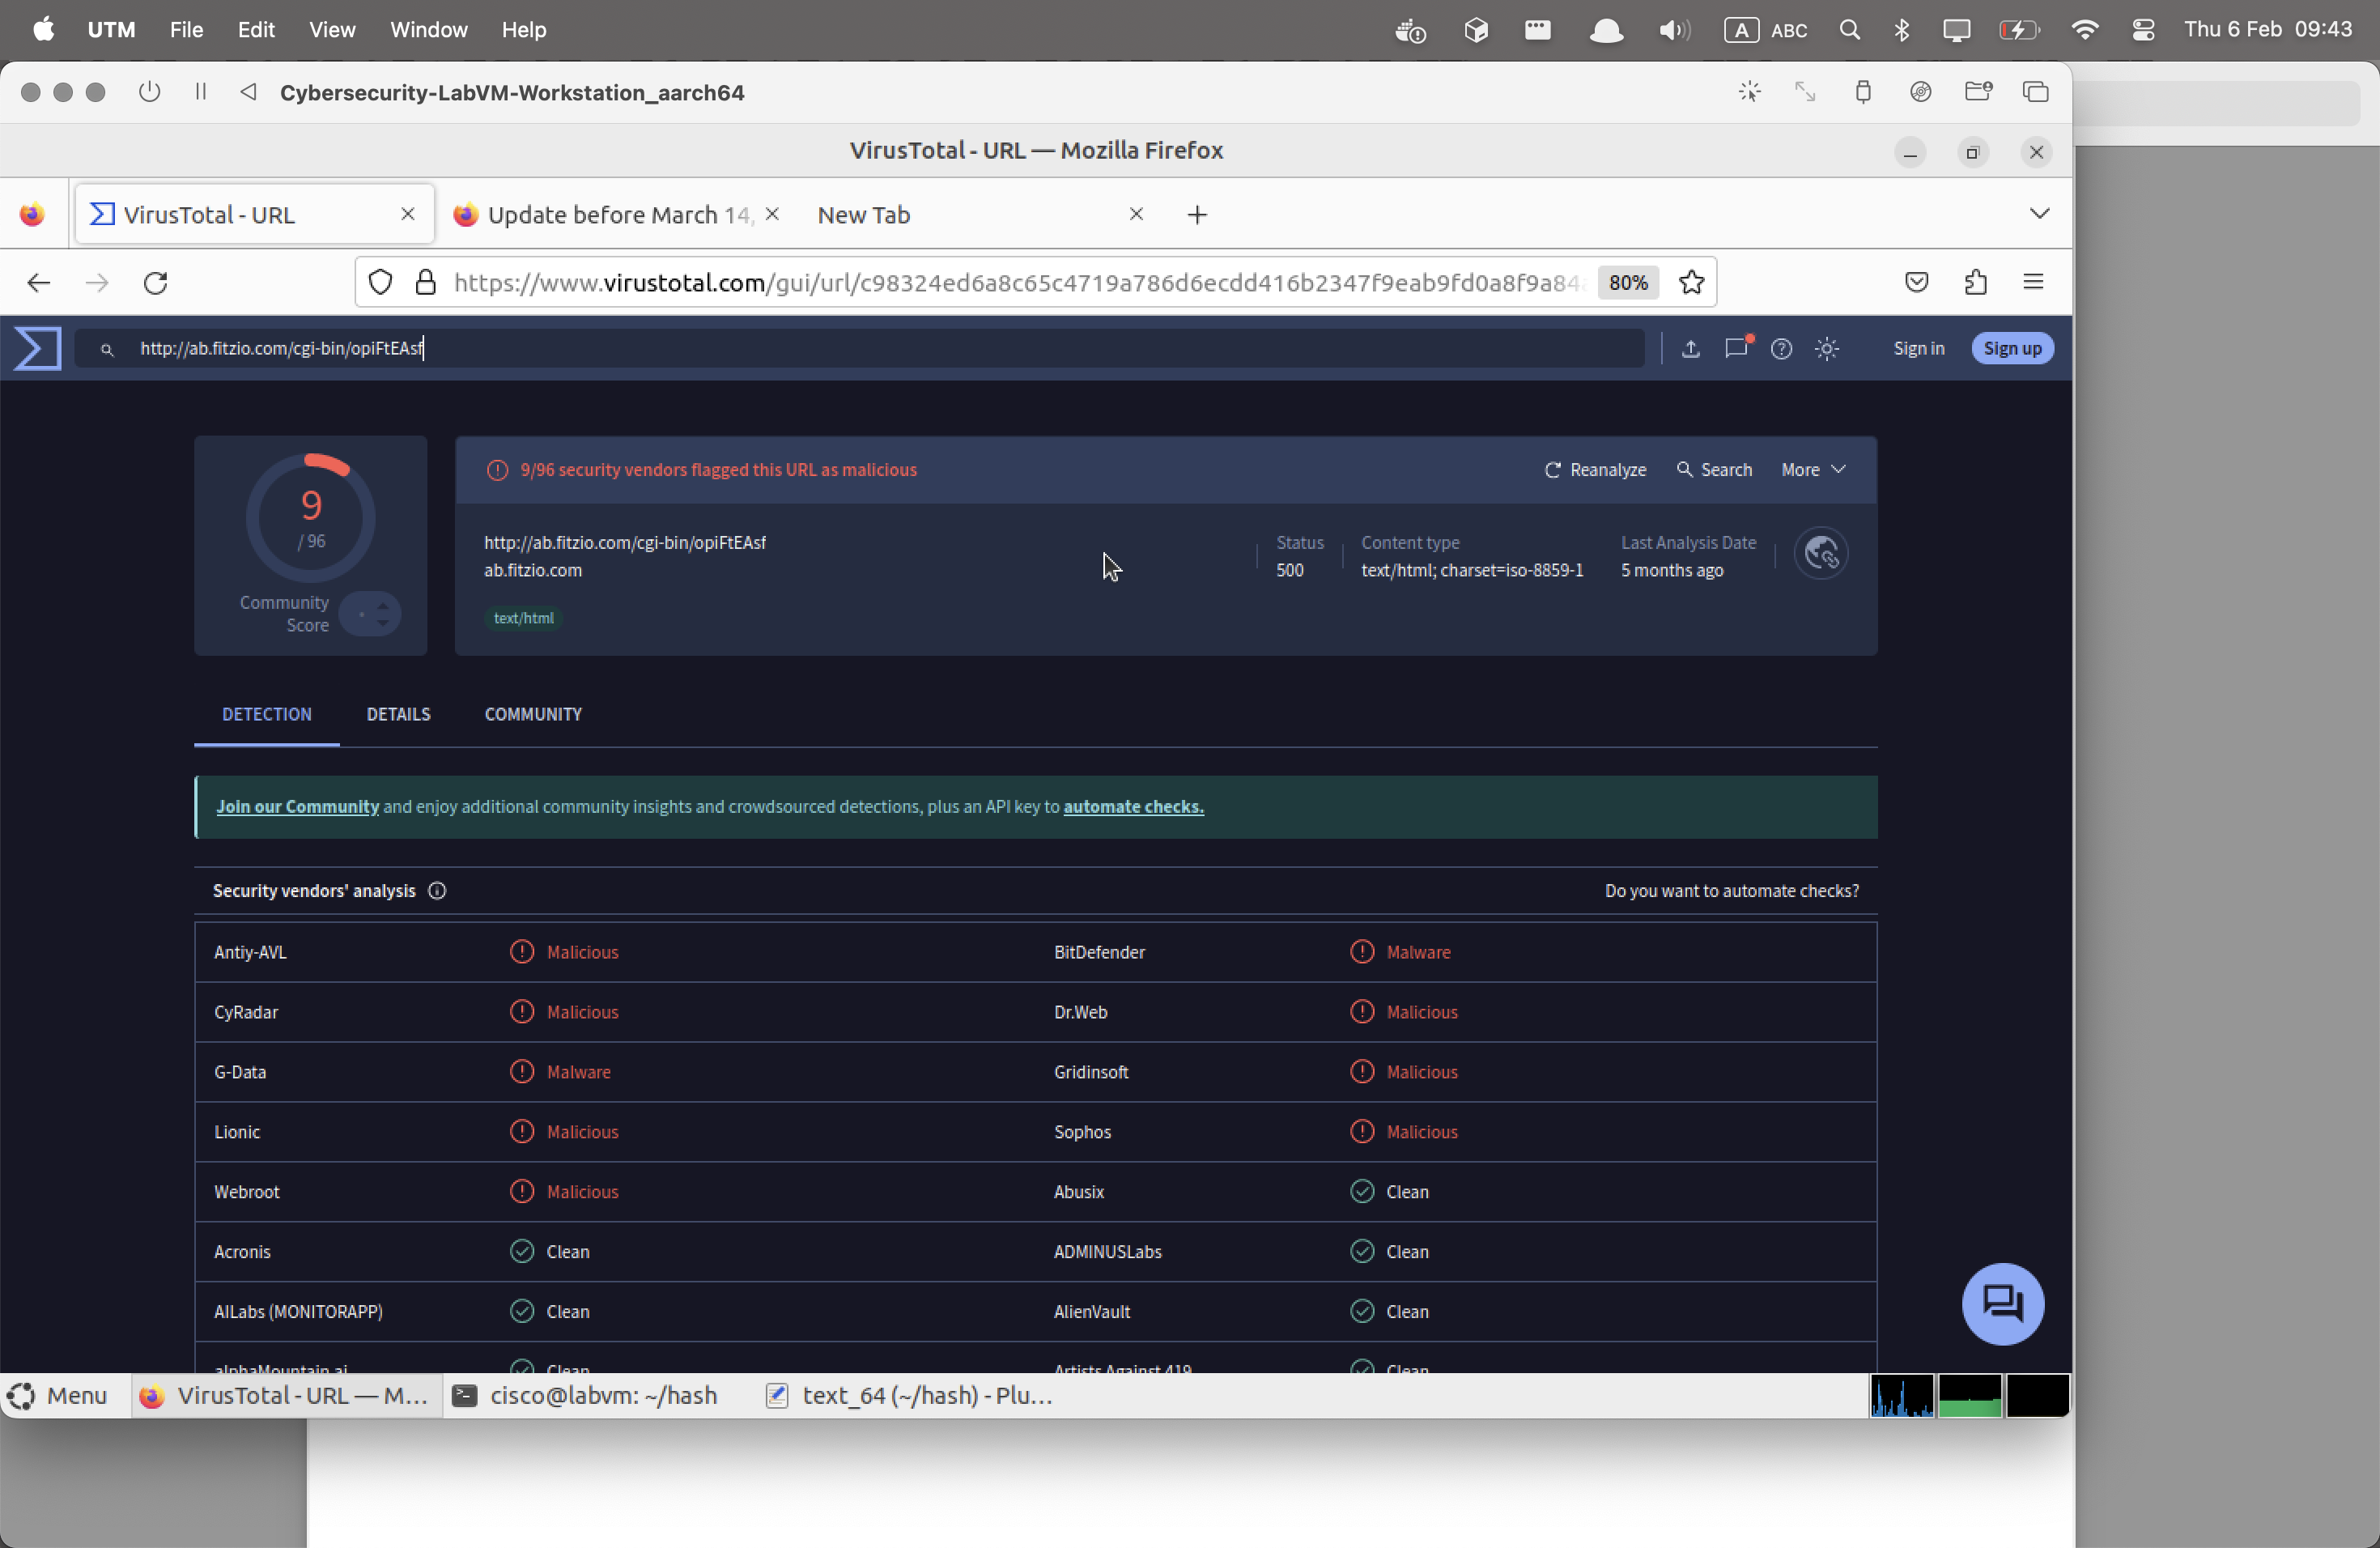
\includegraphics[width=0.9\textwidth]{16.png}

\newpage

\subsubsection*{Note that the variable name, \$tZTLXzZq appears in line four of the code above. Its value is concatenated with the text ‘.exe’.}

\vspace{1\baselineskip}

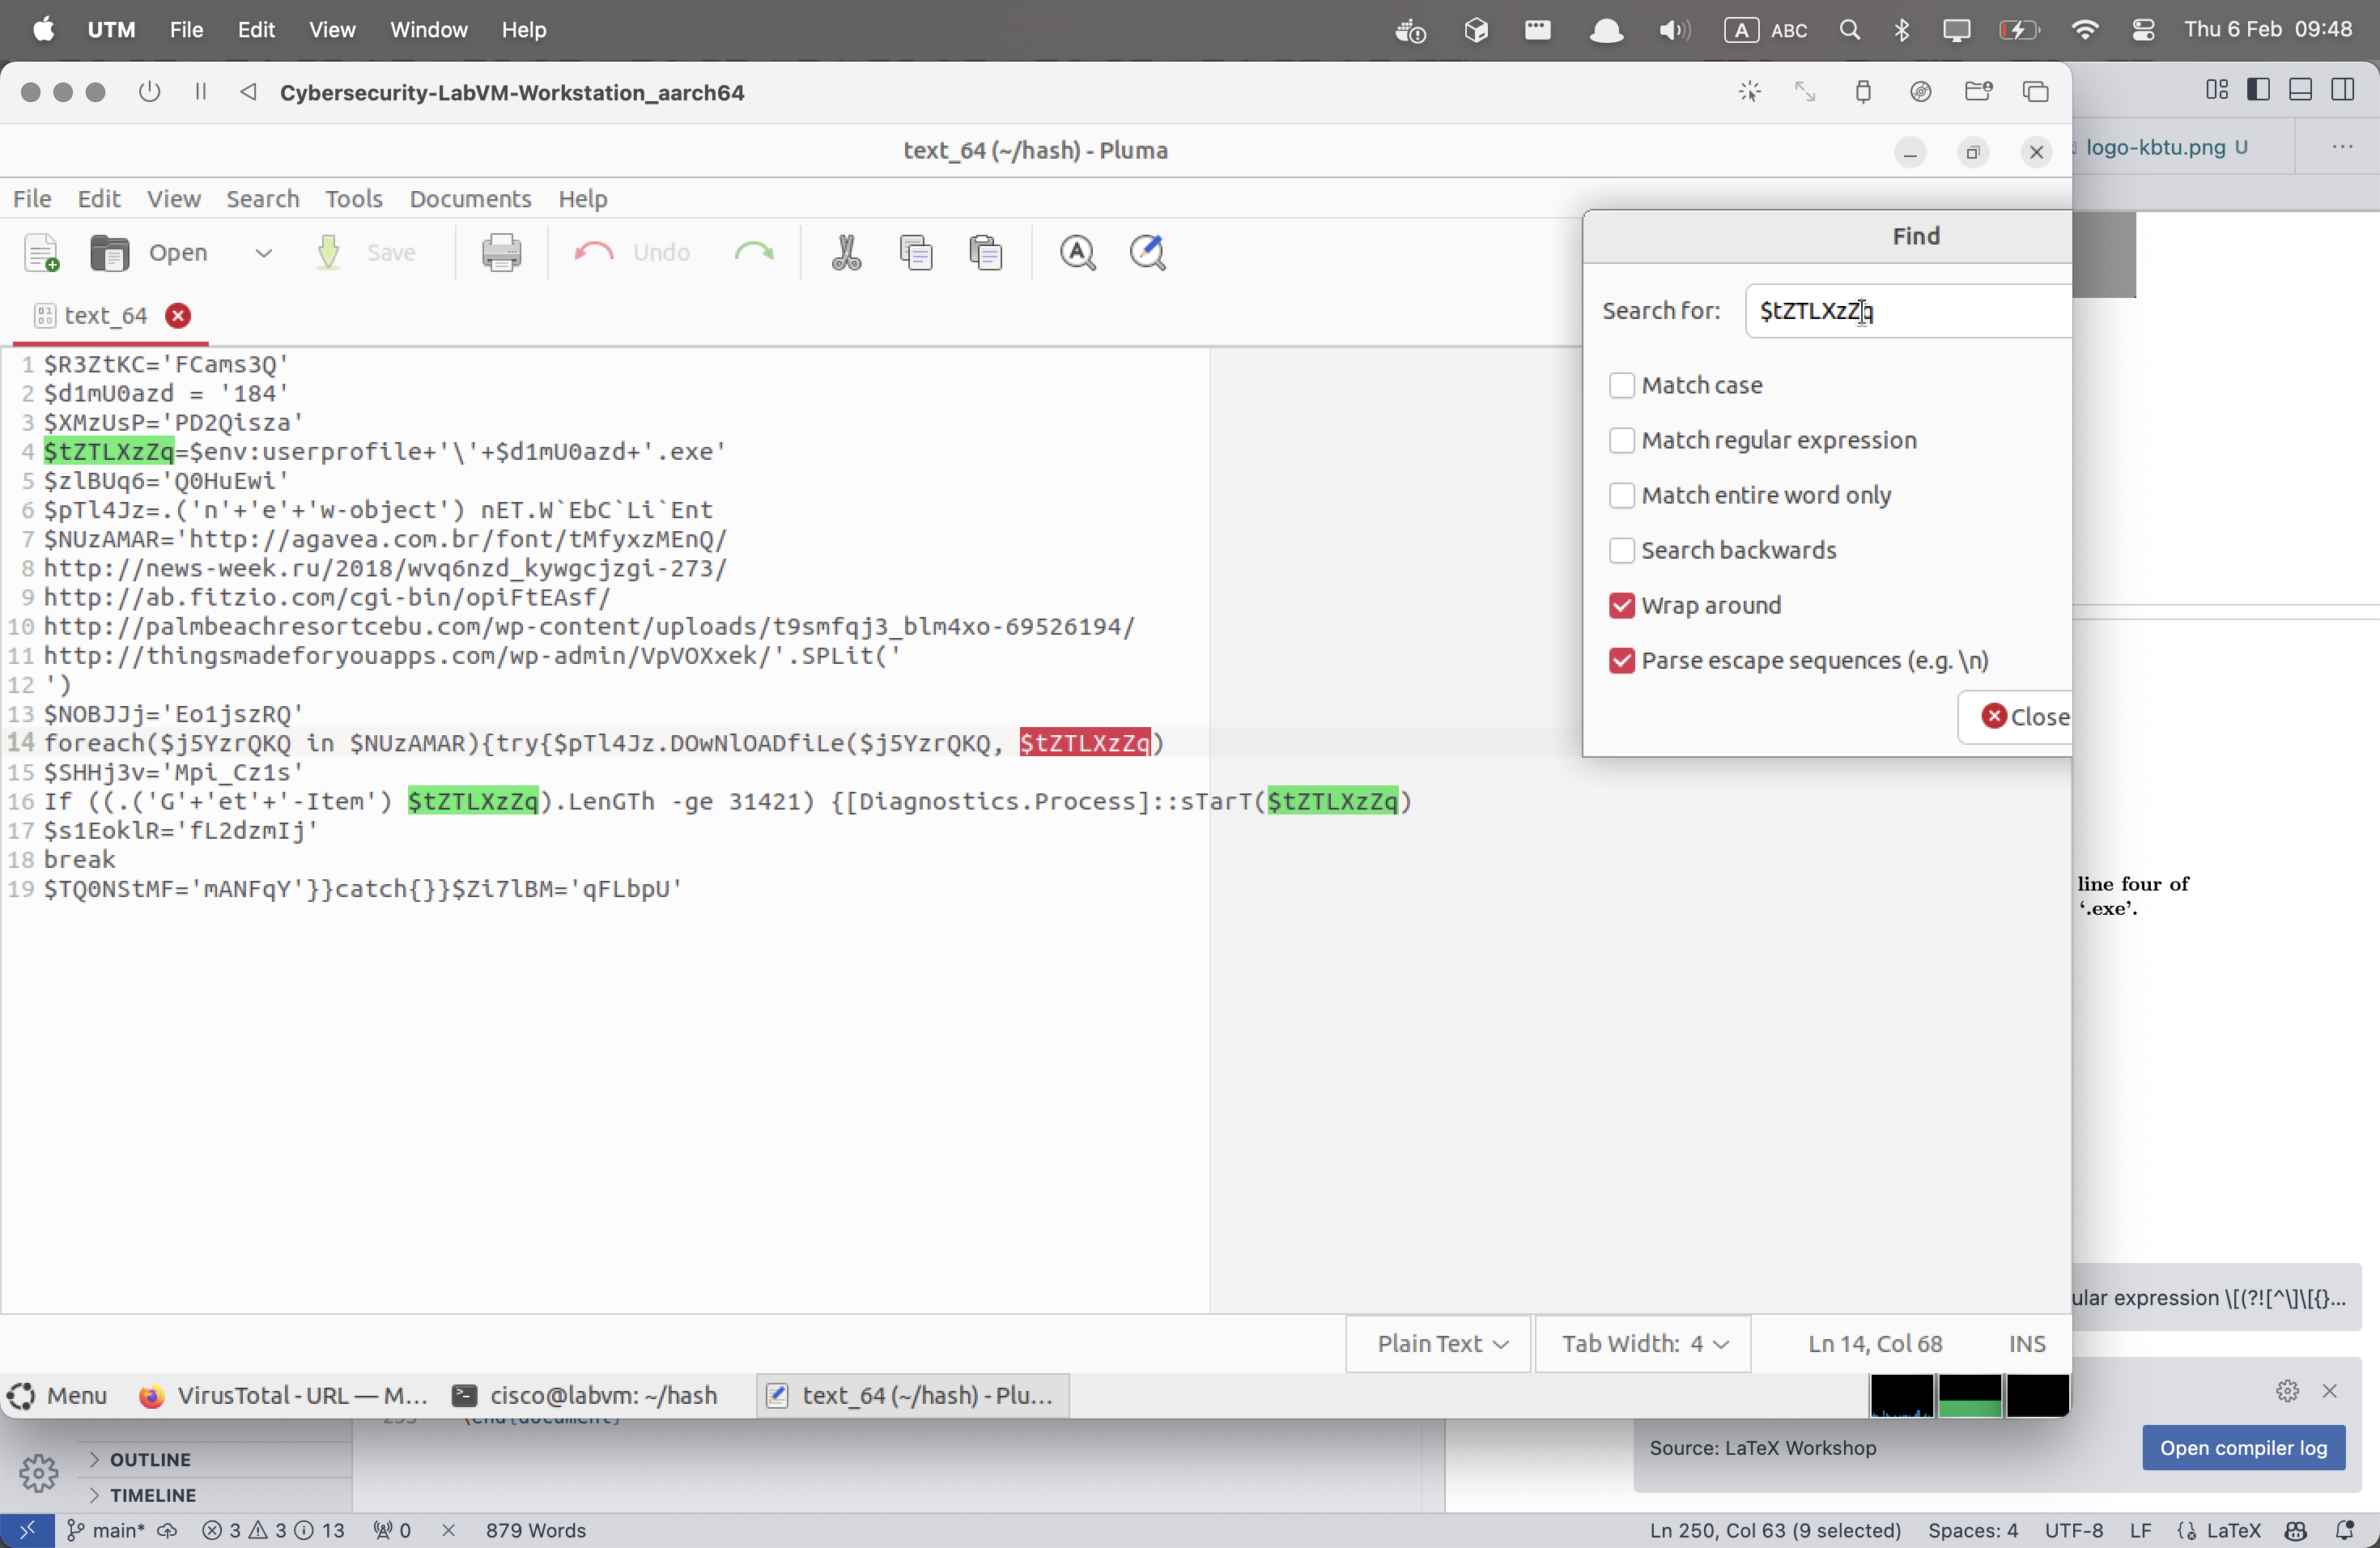
\includegraphics[width=1\textwidth]{17.png}

\vspace{1\baselineskip}

\textbf{\colorbox{yellow}{Question 8: }} What is the value that is assigned to \$tZTLXzZq in line 2? \\
\textbf{Answer: } \$env:userprofile+'\'+\$d1mU0azd+'.exe' \\

\vspace{1\baselineskip}

\textbf{\colorbox{yellow}{Question 9: }} Return to ANY.RUN. What is the next process below powershell? \\
\textbf{Answer: } \texttt{C:\textbackslash Users\textbackslash admin\textbackslash 184.exe}

\vspace{1\baselineskip}

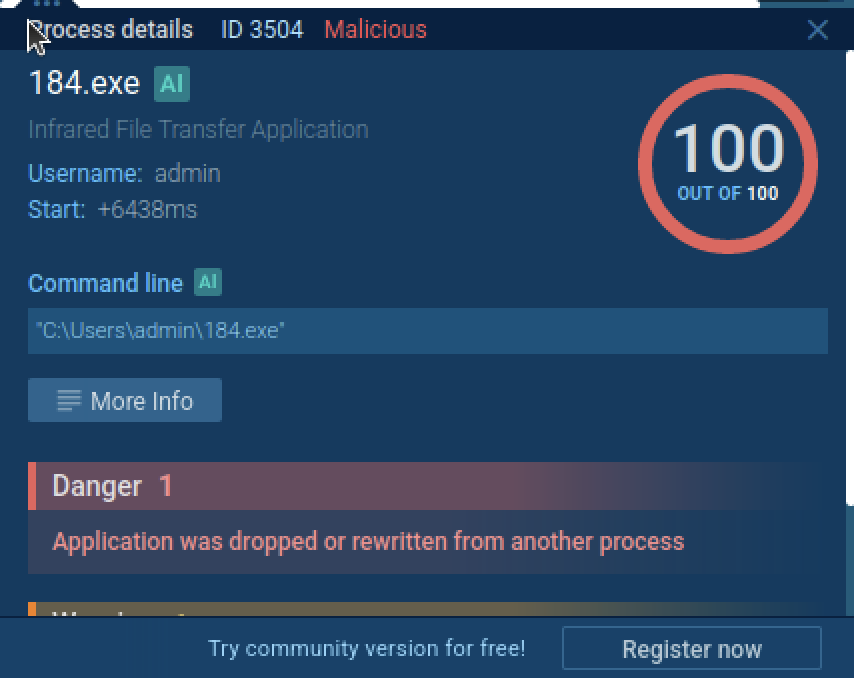
\includegraphics[width=1\textwidth]{18.png}

\vspace{1\baselineskip}

\subsubsection*{Look at line 14. The command is foreach(\$j5YzrQKQ in \$NUzAMAR).}

\vspace{1\baselineskip}

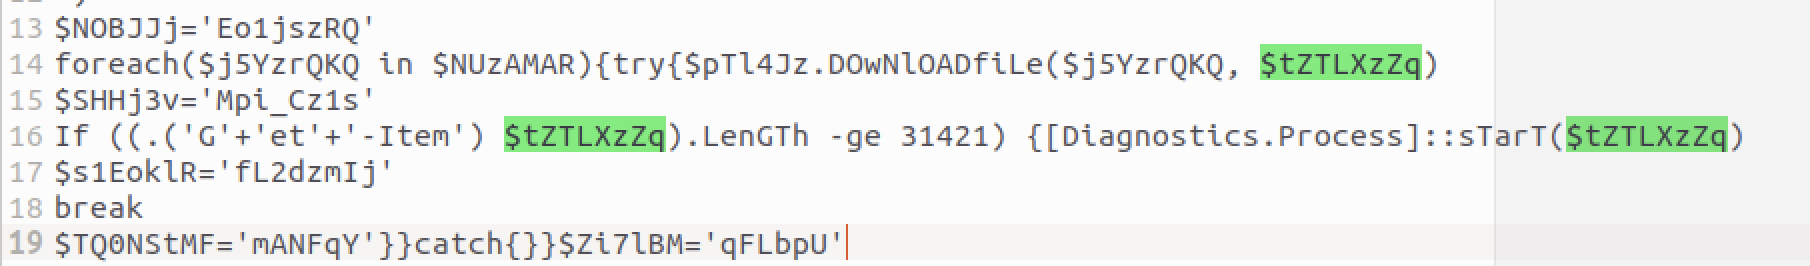
\includegraphics[width=1\textwidth]{19.png}

\vspace{1\baselineskip}

\textbf{\colorbox{yellow}{Question 10: }} What is the contents of the \$NUzAMAR variable as assigned in lines 8 - 11? \\
\textbf{Answer: } 
\$NUzAMAR='\url{http://agavea.com.br/font/tMfyxzMEnQ/} 

\url{http://news-week.ru/2018/wvq6nzd_kywgcjzgi-273/} 

\url{http://ab.fitzio.com/cgi-bin/opiFtEAsf/} \\

\url{http://palmbeachresortcebu.com/wp-content/uploads/t9smfqj3_blm4xo-69526194/}

\url{http://thingsmadeforyouapps.com/wp-admin/VpVOXxek/}'.SPLit('') \newline

\end{document}